% A LaTeX template for ARTICLE version of the MSc Thesis submissions to 
% Politecnico di Milano (PoliMi) - School of Industrial and Information Engineering
%
% S. Bonetti, A. Gruttadauria, G. Mescolini, A. Zingaro
% e-mail: template-tesi-ingind@polimi.it
%
% Last Revision: October 2021
%
% Copyright 2021 Politecnico di Milano, Italy. Inc. NC-BY

\documentclass[11pt,a4paper]{article} 

% ------------------------------------------------------------------------------
%	REQUIRED PACKAGES AND  CONFIGURATIONS
%------------------------------------------------------------------------------
% PACKAGES FOR TITLES
\usepackage{titlesec}
\usepackage{color}

% PACKAGES FOR LANGUAGE AND FONT
\usepackage[utf8]{inputenc}
\usepackage[english]{babel}
\usepackage[T1]{fontenc} % Font encoding

% PACKAGES FOR IMAGES
\usepackage{graphicx}
\graphicspath{{Images/}}
\usepackage{eso-pic} % For the background picture on the title page
\usepackage{subfig} % Numbered and caption subfigures using \subfloat
\usepackage{caption} % Coloured captions
\usepackage{transparent}

% STANDARD MATH PACKAGES
\usepackage{amsmath}
\usepackage{amsthm}
\usepackage{bm}
\usepackage[overload]{empheq}  % For braced-style systems of equations

% PACKAGES FOR TABLES
\usepackage{tabularx}
\usepackage{longtable} % tables that can span several pages
\usepackage{colortbl}

% PACKAGES FOR ALGORITHMS (PSEUDO-CODE)
\usepackage{algorithm}
\usepackage{algorithmic}

% PACKAGES FOR REFERENCES & BIBLIOGRAPHY
\usepackage[colorlinks=true,linkcolor=black,anchorcolor=black,citecolor=black,filecolor=black,menucolor=black,runcolor=black,urlcolor=black]{hyperref} % Adds clickable links at references
\usepackage{cleveref}
\usepackage[backend=biber,style=numeric]{biblatex}
\usepackage{csquotes}
\addbibresource{Thesis_bibliography.bib}

% PACKAGES FOR THE APPENDIX
\usepackage{appendix}

% PACKAGES FOR ITEMIZE & ENUMERATES 
\usepackage{enumitem}

% OTHER PACKAGES
\usepackage{amsthm,thmtools,xcolor} % Coloured "Theorem"
\usepackage{comment} % Comment part of code
\usepackage{fancyhdr} % Fancy headers and footers
\usepackage{lipsum} % Insert dummy text
\usepackage{tcolorbox} % Create coloured boxes (e.g. the one for the key-words)

%-------------------------------------------------------------------------
%	NEW COMMANDS DEFINED
%-------------------------------------------------------------------------
% EXAMPLES OF NEW COMMANDS -> here you see how to define new commands
\newcommand{\bea}{\begin{eqnarray}} % Shortcut for equation arrays
\newcommand{\eea}{\end{eqnarray}}
\newcommand{\e}[1]{\times 10^{#1}}  % Powers of 10 notation
\newcommand{\mathbbm}[1]{\text{\usefont{U}{bbm}{m}{n}#1}} % From mathbbm.sty
\newcommand{\pdev}[2]{\frac{\partial#1}{\partial#2}}
% NB: you can also override some existing commands with the keyword \renewcommand

%----------------------------------------------------------------------------
%	ADD YOUR PACKAGES (be careful of package interaction)
%----------------------------------------------------------------------------
\usepackage{siunitx}
\usepackage[siunitx]{circuitikz}
\usepackage{tikz}
\usetikzlibrary{shapes.geometric, arrows, backgrounds, fit}
\ctikzset{bipoles/length=1.0cm}
\usepackage[autoload=true,
theme=grayscale-plain]{jlcode}

% To use with LuaLatex or XeTeX
% \usepackage{fontspec}

%----------------------------------------------------------------------------
%	ADD YOUR DEFINITIONS AND COMMANDS (be careful of existing commands)
%----------------------------------------------------------------------------


% Do not change Configuration_Files/config.tex file unless you really know what you are doing. 
% This file ends the configuration procedures (e.g. customizing commands, definition of new commands)
% Define blue color typical of polimi
\definecolor{bluepoli}{cmyk}{0.4,0.1,0,0.4}

% Custom theorem environments
\declaretheoremstyle[
  headfont=\color{bluepoli}\normalfont\bfseries,
  bodyfont=\color{black}\normalfont\itshape,
]{colored}

% Set-up caption colors
\captionsetup[figure]{labelfont={color=bluepoli}} % Set colour of the captions
\captionsetup[table]{labelfont={color=bluepoli}} % Set colour of the captions
\captionsetup[algorithm]{labelfont={color=bluepoli}} % Set colour of the captions

\theoremstyle{colored}
\newtheorem{theorem}{Theorem}[chapter]
\newtheorem{proposition}{Proposition}[chapter]

% Enhances the features of the standard "table" and "tabular" environments.
\newcommand\T{\rule{0pt}{2.6ex}}
\newcommand\B{\rule[-1.2ex]{0pt}{0pt}}

% Pseudo-code algorithm descriptions.
\newcounter{algsubstate}
\renewcommand{\thealgsubstate}{\alph{algsubstate}}
\newenvironment{algsubstates}
  {\setcounter{algsubstate}{0}%
   \renewcommand{\STATE}{%
     \stepcounter{algsubstate}%
     \Statex {\small\thealgsubstate:}\space}}
  {}

% New font size
\newcommand\numfontsize{\@setfontsize\Huge{200}{60}}

% Title format: chapter
\titleformat{\chapter}[hang]{
\fontsize{50}{20}\selectfont\bfseries\filright}{\textcolor{bluepoli} \thechapter\hsp\hspace{2mm}\textcolor{bluepoli}{|   }\hsp}{0pt}{\huge\bfseries \textcolor{bluepoli}
}

% Title format: section
\titleformat{\section}
{\color{bluepoli}\normalfont\Large\bfseries}
{\color{bluepoli}\thesection.}{1em}{}

% Title format: subsection
\titleformat{\subsection}
{\color{bluepoli}\normalfont\large\bfseries}
{\color{bluepoli}\thesubsection.}{1em}{}

% Title format: subsubsection
\titleformat{\subsubsection}
{\color{bluepoli}\normalfont\large\bfseries}
{\color{bluepoli}\thesubsubsection.}{1em}{}

% Shortening for setting no horizontal-spacing
\newcommand{\hsp}{\hspace{0pt}}

\makeatletter
% Renewcommand: cleardoublepage including the background pic
\renewcommand*\cleardoublepage{%
  \clearpage\if@twoside\ifodd\c@page\else
  \null
  \AddToShipoutPicture*{\BackgroundPic}
  \thispagestyle{empty}%
  \newpage
  \if@twocolumn\hbox{}\newpage\fi\fi\fi}
\makeatother

%For correctly numbering algorithms
\numberwithin{algorithm}{chapter}

\lstdefinestyle{juliacode}{
  language=Julia, 
  showstringspaces=false,
  numbers=left,
  % stepnumber=1,
  numberstyle=\tiny,
  stepnumber=2,
  % numbersep=10pt,
  % Comment the following three lines to remove colors
  keywordstyle=\color{blue},
  commentstyle=\color{gray},
  identifierstyle=\color{purple!80},
  columns=fullflexible,
  keepspaces=true
}

\lstnewenvironment{juliacode}{\lstset{style=juliacode}}{}

%% To use with LuaLatex or XeTeX
% \newfontfamily \JuliaMono {JuliaMono-Light.ttf}[
%     Path      = ./,
%     Extension = .ttf
%     ]
% \newfontface \JuliaMonoLight{JuliaMono-Light}
% \setmonofont{JuliaMono-Light}[ Contextuals=Alternate ]

\tikzstyle{startstop} = [rectangle, rounded corners, minimum width=2cm, text width=3cm, minimum height=1cm,text centered, draw=black, fill=red!30]
\tikzstyle{process}   = [rectangle, minimum width=2cm, text width=3cm, minimum height=1cm, text centered, draw=black, fill=orange!30]
% \tikzstyle{process}   = [rectangle, draw=black, text width=3cm, fill=orange!30]
\tikzstyle{decision}  = [diamond, minimum width=2cm, minimum height=1cm, text centered, draw=black, fill=green!30]
\tikzstyle{image}     = [minimum width=1cm, minimum height=1cm, text centered]
\tikzstyle{arrow}     = [thick,->,>=stealth]

% Insert here the info that will be displayed into your Title page 
% -> title of your work
\renewcommand{\title}{Simulating Aeration at Birth: building an Open-Source Newborn Lung Model}
% -> author name and surname
\renewcommand{\author}{Luca Andriotto}
% -> MSc course
\newcommand{\course}{Biomedical Engineering - Ingegneria Biomedica}
% -> advisor name and surname
\newcommand{\advisor}{Prof. Raffaele Dellacà}
% IF AND ONLY IF you need to modify the co-supervisors you also have to modify the file Configuration_Files/title_page.tex (ONLY where it is marked)
\newcommand{\firstcoadvisor}{Dr. Chiara Veneroni} % insert if any otherwise comment
\newcommand{\secondcoadvisor}{} % insert if any otherwise comment
% -> author ID
\newcommand{\ID}{928454}
% -> academic year
\newcommand{\YEAR}{2023-2024}
% -> abstract (only in English)
\renewcommand{\abstract}{During pregnancy, the fetal airways are
filled with a fluid known as fetal lung fluid, which is essential for
the development of airway width. Consequently, at birth, the
respiratory system must expel this fluid to allow air to enter and
exit, a process necessary for breathing (aeration). Fluid reabsorption
begins a few days before birth through chemical processes involving
sodium channels, and during natural childbirth, fluid is expelled from
the mouth and nose due to the compression of the neonate's chest. In
full-term infants, the likelihood of complications during aeration is
very low. However, the scenario is vastly different for preterm
infants, who are born before 37 weeks of gestation compared to the
typical 40 weeks of a normal pregnancy.  Although recruitment
maneuvers have gained more interest in preterm ventilation, there is
still no common medical strategy. Experimental procedures are tested
on animals, presenting challenges in obtaining results due to the
invasiveness of the procedures and associated ethical issues. In
silico modeling of the adult lung has been useful for understanding
pathophysiology and making diagnoses. Thus, the same approach could
help analyze various recruitment strategies and their impact on the
lung during initial aeration at birth. However, in silico models of
neonatal lungs are limited to describing up to the first generation of
the bronchial tree and are therefore inadequate for simulating the
physiological changes that occur at birth.}

% -> key-words (only in English)
\newcommand{\keywords}{morphometric model, aeration process,
lung, newborn, respiratory system}



%%% Local Variables:
%%% mode: LaTeX
%%% TeX-master: "Thesis"
%%% TeX-engine: luatex
%%% End:


%%%%%%%%%%%%%%%%%%%%%%%%%%%%%%
%%     THESIS MAIN TEXT     %%
%%%%%%%%%%%%%%%%%%%%%%%%%%%%%%

\begin{document}

%-----------------------------------------------------------------------------
% TITLE PAGE
%-----------------------------------------------------------------------------
% DO NOT REMOVE SPACES BETWEEN LINES!

\twocolumn[{\begin{@twocolumnfalse}

\AddToShipoutPicture*{\BackgroundPic}

\hspace{-0.6cm}
\includegraphics[width=0.6\textwidth]{logo_polimi_ing_indinf.eps}

\vspace{-1mm}
\fontsize{0.3cm}{0.5cm}\selectfont \bfseries \textsc{\color{bluePoli} Executive Summary of the Thesis}\\

\vspace{-0.2cm}
\Large{\textbf{\color{bluePoli}{\title}}}\\

\vspace{-0.2cm}
\fontsize{0.3cm}{0.5cm}\selectfont \bfseries \textsc{\color{bluePoli} Laurea Magistrale in \course}\\

\vspace{-0.2cm}
\fontsize{0.3cm}{0.5cm} \selectfont \bfseries Author: \textsc{\textbf{\author}}\\

\vspace{-0.4cm}
\fontsize{0.3cm}{0.5cm}\selectfont \bfseries Advisor: \textsc{\textbf{\advisor}}\\

% if only ONE co-advisor is present:
\vspace{-0.4cm}
\fontsize{0.3cm}{0.5cm}\selectfont \bfseries Co-advisor: \textsc{\textbf{\firstcoadvisor}}\\
% if more than one co-advisors are present:
%\vspace{-0.4cm}
%\fontsize{0.3cm}{0.5cm}\selectfont \bfseries Co-advisors: \textsc{\textbf{\firstcoadvisor}}\textsc{\textbf{\secondcoadvisor}}\\

\vspace{-0.4cm}
\fontsize{0.3cm}{0.5cm}\selectfont \bfseries Academic year: \textsc{\textbf{\YEAR}}

\small \normalfont

\vspace{11pt}

\centerline{\rule{1.0\textwidth}{0.4pt}}

\vspace{15pt}
\end{@twocolumnfalse}}]

\thispagestyle{plain} % In order to not show the header in the first page

%-----------------------------------------------------------------------------
% TOC
%-----------------------------------------------------------------------------

% 1. Introduction
% 2. Capitolo sul Polmone dei Neonati (non visibile)
% 3. Anatomical Models
%   3.1. Existing Infant Lungs Models
% 4. Mechanical model of airways and acini
% 5. Model Development
%   5.1. Airway Tree
%     5.1.1. CT Image Processing: Lung Segmentation, Centerline and Radii Extraction
%     5.1.2. Generation of the Statistical Portion
%   5.2. Mechanical Simulator
%     5.2.1. Blocks Description
%     5.2.2. Callbacks' Role in State Variables Discontinuity Handling
%     5.2.3. Model Testing on A Subtree
% 6. Results and Validations  
%   6.1. Anatomical Surrogate
%   6.2. Mechanical Simulation
% 7. Discussion and Conclusion

% -----------------------------------------------------------------------------
% CHAPTERS
%-----------------------------------------------------------------------------
% 1. Introduction
\section{Introduction}
\label{sec:introduction}

During pregnancy, the fetal airways are filled with a fluid known as
fetal lung fluid, which is essential for the development of airway
width. Consequently, at birth, the respiratory system must expel this
fluid to allow air to enter and exit, a process necessary for
breathing (aeration). Fluid reabsorption begins a few days before
birth through chemical processes involving sodium channels, and during
natural childbirth, fluid is expelled from the mouth and nose due to
the compression of the neonate's chest. In full-term infants, the
likelihood of complications during aeration is very low. However, the
scenario is vastly different for preterm infants, who are born before
37 weeks of gestation compared to the typical 40 weeks of a normal
pregnancy.

Applying pressure at the entrance of the airways helps preterm infants
remove the fluid and open the closed acini. Once the acini are
recruited, less pressure is needed to keep them open and ventilate the
lung. Thus, employing recruitment strategies at birth has the
advantage of initiating ventilation in a more recruited lung, using
lower pressures, achieving more homogeneous lung aeration, and
reducing the stress applied to the tissues. It is important to note,
however, that at birth, the lung is more delicate and thus more
susceptible to damage, even with routine ventilation
procedures. Therefore, developing protective recruitment strategies at
birth could lead to significant improvements in this area.

Although recruitment maneuvers have gained more interest in preterm
ventilation, there is still no common medical strategy. Experimental
procedures are tested on animals, presenting challenges in obtaining
results due to the invasiveness of the procedures and associated
ethical issues\cite{al-jumaily2011, herrmann2016}. In silico modeling
of the adult lung has been useful for understanding pathophysiology
and making diagnoses. Thus, the same approach could help analyze
various recruitment strategies and their impact on the lung during
initial aeration at birth. However, in silico models of neonatal lungs
are limited to describing up to the first generation of the bronchial
tree resulting inadequate for simulating the physiological changes
that occur at birth.  Anatomical models of the adult lung were scaled
to match the newborns one. However, there are differences between
airway length and diameter proportion between infants and
adults\cite{horsfield1987}. Moreover, the immature lung structure
results in different mechanical properties\cite{merkus1996}.

% AGGIUNTA MODIFICA, COMPLETARE
Alternatively, anatomical properties .. scaled r.

Consequently, both the anatomical and mechanical characteristics of
the tissues must be appropriately modified to achieve a consistent
model for the neonatal case in the time domain.  Finally, to implement
the changes occurring at birth, the mechanical properties of each
airway must change when the fetal fluid is replaced by air.

A previous thesis work developed an in silico model able to simulate
the mechanical changes occurring in the airways during aeration at
birth in the time domain. However, the anatomical structure was scaled
for the adult one, and the mechanical model was implemented in
"CADENCE.", a platform optimised for the analysis of integrated
circuits. The use of «CADENCE» platform results in limitations related
to the need for proprietary software licenses and difficulties in
implementing time-varying phenomena not easily described by standard
electronic components.

Using open-source strategies for the model eliminates the need for
proprietary software licenses, making the development process more
accessible\cite{mani2020}.


Aims of this projects are:
\begin{description}
\item Generate a model from neonatal CT scans to optimize the
  generation of airways, ensuring they adhere to the morphometric
  characteristics at various ages.
\item Develop an open-source mechanical model that allows for the
  simulation of mechanical properties along with fluid dynamics
  \cite[][Ch. 1.9 - 1.11]{mani2020} (capillary pressure associated
  with the air-fluid interface).
\end{description}

%%% Local Variables:
%%% mode: LaTeX
%%% TeX-master: "../Thesis"
%%% End:

% % 2. Methods
%   2.1. Chaste
%   2.2. Morphometric model
%     2.2.1. CT image processing: lung segmentation, centerline and radii extraction
%     2.2.2. Generation of the statistical part
%   2.3. Julia Programming Language
%     2.3.1. «ModelingToolkit.jl» handles model complexity
%     2.3.2. Callbacks role in state variables discontinuity handling
%   2.4. Mechanical model
%     2.4.1. Blocks description
%     2.4.2. Model testing on a subtree

% 2. Methods
\section{Methods}
% Visione d'insieme (diagramma con flusso dell'informazione, data
% pipeline). Questo diagramma mostra a partire dagli input che ho
% avuto (TC) tutto l'iter del dato.

% Qui ha detto poi Chiara che conviene inserire delle informazioni
% riguardanti i modelli matematici utilizzati.

\Cref{fig:data_pipeline} provides a high-level overview of the main
operations performed.  Each of the two classes of methods correspondss
to one of the two models:

\begin{enumerate}
\item \emph{Chaste} library is utilized in the generation of
  \emph{morphometric model}.
\item \emph{Julia Programming Language} is employed to describe and
  instantiate the \emph{mechanical model}, as well as to perform
  \emph{simulations}.
\end{enumerate}

% todo: modificare l'immagine sopra ad "anatomical surrogate generation" con uno screen di ParaView.
% todo: aggiungere immagini sopra al branch del modello meccanico.

\begin{figure}[H]\centering
  \begin{tikzpicture}[node distance=3cm]
    % Nodes
    %% Chaste & Morphometric Model
    \node (ct_acquisition)           [startstop] {CT\\Acquisition};
    \node (img_ct_acquisition)       [image, above of=ct_acquisition, yshift=-1.0cm]                   {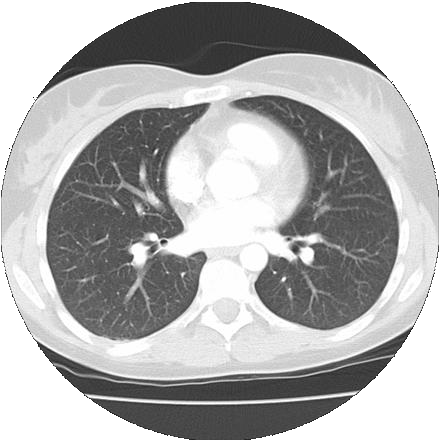
\includegraphics[width=2.0cm]{ct_acquisition.png}};
    %%% Upper branch
    \node (lobes_segmentation)       [process, right of=ct_acquisition, xshift=3.25cm, yshift=+2cm]    {Lobes\\segmentation};
    %%% Lower branch
    \node (img_lobes_segmentation)   [image, above of=lobes_segmentation, xshift=-.1cm, yshift=-1.2cm] {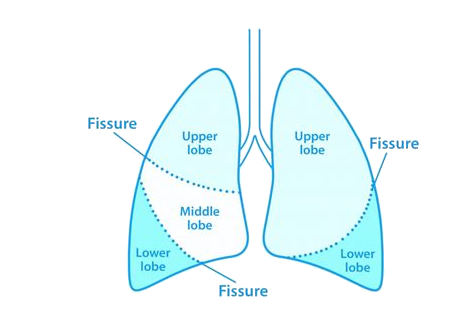
\includegraphics[width=3.5cm]{lobes_segmentation.png}};
    \node (airways_segmentation)     [process, below of=lobes_segmentation, xshift=-2cm, yshift=-1cm]  {Airways\\segmentation};
    \node (img_airways_segmentation) [image, above of=airways_segmentation, xshift=2cm, yshift=-1cm]   {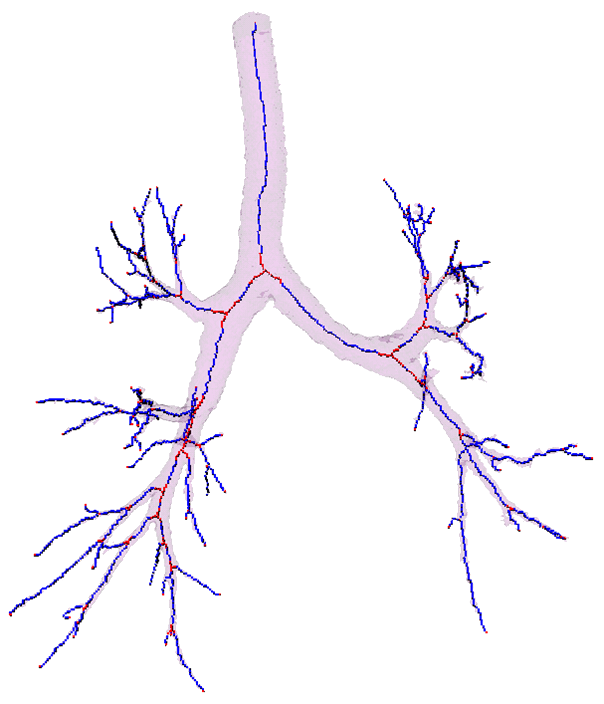
\includegraphics[height=2.5cm]{airways_segmentation.png}};
    \node (centerline_extraction)    [process, below of=lobes_segmentation, xshift=+2cm, yshift=-1cm]  {Centerline\\extraction};
    \node (surrogate_generation)     [process, right of=ct_acquisition, xshift=9.5cm]                  {Anatomical surrogate\\generation};
    \node (img_surrogate_generation) [image, above of=surrogate_generation, yshift=-.5cm]              {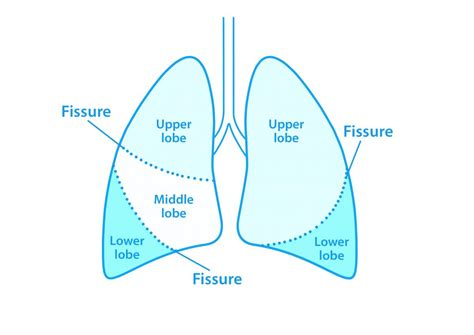
\includegraphics[width=3.5cm]{lobes_segmentation.jpg}};
    %% Julia & Mechanical Model
    \node (parameters_update)        [process, below of=ct_acquisition, yshift=-3cm]                   {Lungs parameters\\update};
    \node (model_instantiation)      [process, right of=parameters_update, xshift=1cm]                 {Mechanical model\\instantiation};
    \node (DAE_solution)             [process, right of=model_instantiation, xshift=1cm]               {DAE System\\solution};
    \node (simulations)              [startstop, right of=DAE_solution, xshift=+1cm]                   {Mechanical Simulations};

    % Arrows
    \draw [arrow] (ct_acquisition.east)                              -- ++(.5,0) coordinate(tmp)     |- (airways_segmentation.west);
    \draw [arrow] (airways_segmentation)                             -- (centerline_extraction);
    \draw [arrow] (centerline_extraction.east)                       -- ++(.5,0) coordinate(tmp1)    |- (surrogate_generation.west);
    \draw [arrow] (model_instantiation)                              -- (DAE_solution);
    \draw [arrow] (DAE_solution)                                     -- (simulations);
    \draw [arrow] (tmp)                                              |-   (lobes_segmentation.west);
    \draw [arrow] (lobes_segmentation)                               --   (tmp1|-lobes_segmentation) |- (surrogate_generation.west);
    \draw [dashed, thick, ->,>=stealth] (surrogate_generation.south) -- ++(0,-3.5)                   -| (parameters_update.north);
    \draw [arrow] (parameters_update)                                -- (model_instantiation);

    % Frame around a part of the flowchart
    \begin{pgfonlayer}{background}
      \node[rounded corners=3mm,
      draw=blue,
      thick, dashed,
      fit=(airways_segmentation)(centerline_extraction)(img_lobes_segmentation)(img_surrogate_generation),
      fill=cyan!5,
      inner sep=7pt,
      label={[anchor=north]below:\textsc{\textcolor{blue}{Chaste \& Morphometric model}}}] {};
    \end{pgfonlayer}
    \begin{pgfonlayer}{background}
      \node[rounded corners=3mm,
      draw=red,
      thick, dashed,
      fit=(parameters_update)(model_instantiation)(DAE_solution),
      fill=magenta!5,
      inner sep=7pt,
      label={[anchor=north]below:\textsc{\textcolor{red}{Julia Programming Language \& Mechanical model}}}] {};
    \end{pgfonlayer}
  \end{tikzpicture}
  \caption{Data pipeline.  The process begins with a
    \emph{patient-specific image} (i.e. CT) of a premature newborn.
    The extracted data, comprising \emph{two segmentations}, are then
    processed to obtain an anatomical surrogate of the airway tree.
    This is necessary due to scanner resolution not allowing for the
    discrimination and localization of small branches.  From the
    resulting morphometric model, the \emph{mechanical parameters} can
    be derived, which are essential for generating an accurate
    simulation model.  Finally, a numerical solver for differential
    equations provides the final output.}
    \label{fig:data_pipeline}
\end{figure}

%%% Local Variables:
%%% mode: LaTeX
%%% TeX-master: "../Thesis"
%%% End:


%   2.1. Chaste
\subsection{Chaste}
\label{subsec:chaste}

Chaste is a C++ open-source (BSD licensed) library developed by Oxford
University.  It has multiple use cases across various biomedical
fields, with an emphasis on cardiac electrophysiology and cancer
development\cite{mirams2013}.  It can be integrated into a C++ program
or used via «User Project» (i.e. \texttt{ctest}).
Specifically, the ``AirwayGenerationTutorial'' is considered as a
first codebase and properly adapted to match newborn
parameters\cite{airwaygeneration2024}.

The required input consists of two pieces of information:
\begin{itemize}
\item A \emph{mesh of centerline points}.  This mesh is provided in
  TetGen format, comprising ``airways.node'' and ``airways.edge''
  files. The first file lists centerline points coordinates,
  respective sampled airways radius and a boolean value to indicate if
  the point is generative. The second one contains all the connections
  between pairs of points.
\item Four (or five) \emph{lobes segmentations} in STL format.  These
  segmentations are necessary as they physically impose a limit on the
  growth algorithm.
\end{itemize}

%   2.2. Morphometric model
\subsection{Morphometric Model}
\label{subsec:morphometric_model}
% Per Chiara: Inserisco definizione di modello morfometrico?

%     2.2.1. CT, centerline and radii extraction
\subsubsection{CT Image Processing: Lung Segmentation, Centerline and
  Radii Extraction}
\label{subsubsec:ct_centerline_radii_extraction}
% todo: Devo chiedere bene a Francesca come sono stati estratti i
% raggi.

«3D Slicer» is an open-source software used for CT image processing.
Two extensions are installed:

\begin{description}
\item «\emph{Chest\_imaging\_platform}»: This extension enables
  semi-automatic segmentation of major airways from a single fiducial
  point.  It can also extract adult lobes using three fiducial points
  per lung fissure. However, in our case, the fissures are not
  visible, necessitating manual intervention.
\item «\emph{SlicerVMTK}»: This extension is used for extracting
  centerline points.
\end{description}

%     2.2.2. Generation of the statistical part
\subsubsection{Generation of the Statistical Portion}
\label{subsubsec:statistical_generation}

% Riferirsi a Tawhai2000.

The Chaste User Project reads the input files (see
\Cref{subsec:chaste}), and begins growing the anatomical surrogate
from the points labeled as «generative».  The algorithm operating
under the hood is a modified version of the one described in
\cite{tawhai2000}.  The generated output is available in various
formats:

\begin{itemize}
\item vtu: Unstructured Grid (base64 encoded) format used by VTK
  library.  It can be displayed by ParaView, an open-source viewer.
\item node and edge: TetGen format.  Such files are better suited for
  further processing.
\end{itemize}

%   2.3. Julia Programming Language
\subsection{Julia Programming Language}
\label{subsec:julia}

Julia is a free, open-source (MIT licensed), fast, scientific and
numerical computing-oriented programming language.  Its computational
efficiency is comparable to that of statically-typed languages like C
or Fortran.  Moreover, its high-level code expressivity rivals that of
languages like Python, R and MATLAB\cite{juliadocs2024}.

Two key features, inspired by the \emph{Lisp Language}, are
highlighted here.

\begin{description}
\item \emph{Metaprogramming}: Code is treated as any other Julia data
  structure, thus can be dynamically generated and manipulated at
  runtime.
\item \emph{Macros}: They help instantiate the generated code in the
  body of a program.
\end{description}

Their importance is closely tied to the concept of Domain-Specific
Languages (aka DSLs).  These dialects are composed by abstractions
that can be properly exploited to solve particular problems
(e.g. modeling complex systems, solving differential equations).

Julia REPL has a built-in package manager (i.e. «\texttt{Pkg.jl}»)
used for managing project dependencies and ensuring the
\emph{repeatability} of computational setups.  This is achieved by
saving the required package names and commits into `Project.toml' and
`Manifest.toml' files.

%     2.3.1. «ModelingToolkit.jl» handles model complexity
\subsubsection{«\texttt{ModelingToolkit.jl}» handles
  Model Complexity}
\label{subsubsec:modelingtoolkit}

This Julia package encompasses all the tools necessary for model
design.  \texttt{ModelingToolkit.jl}» is equation-driven, requiring
each system to be described by Differential-Algebraic Equations
(i.e. DAEs) for subsequent solving\cite{ma2021}. Its built-in DSL
optimizes every stage of modeling, from prototyping components to
instantiating the complete system.

An acausal paradigm can be adopted, allowing users to reason in terms
of \emph{components}\cite{mtkdocs2024}. This modularity facilitates
system extensibility compared to the causal approach, where the entire
system of Differential-Algebraic Equations must be considered and
manually simplified\cite{ma2024}.

In particular, the usage of \jlinl{@mtkmodel} macro enables
hierarchical generation of building blocks recurring in the
highest-order model (i.e. «Lungs»).  Here is how information is
structured within \jlinl{@mtkmodel} macro.

\begin{jllisting}[label=@mtkmodel, caption={\jlinl{@mtkmodel}: a macro for systems prototyping.}]
  @mtkmodel <name_of_model> begin
      @parameters begin
          # (Optional) Some constant (e.g. Resistance, Capacitance) ...
      end
      @components begin
          # (Optional) Some dependency system (e.g. Resistor, Capacitor) ...
      end
      @variables begin
          # (Optional) Internal variables ...
      end
      @equations begin
          # Differential Algebraic Equations describing the model's behavior.
      end
      @continuous_events begin
          # (Optional) Some callback function ...
      end
  end
\end{jllisting}

Replicating the behavior of electrical components using this language
is straightforward, once you are familiar with the syntax and
understand the Differential-Algebraic Equations that represent their
characteristics.  Each generated system can then be composed into more
complex ones, using the internal \jlinl{@components} macro, thereby
implementing the hierarchical structure mentioned earlier.

After describing the highest-order system, Julia compiler requires its
instantiation before any simulation can be performed.  This is
accomplished using \jlinl{@mtkbuild} macro, which minimizes the number
of equations that need to be solved.

%     2.3.2. Callbacks role in state variables discontinuity handling
\subsubsection{Callbacks' Role in State Variables Discontinuity
  Handling}
\label{subsubsec:callbacks}

Not all characteristics of electrical components can be defined solely
by DAEs.  Voltages or currents may suddently change, triggered by a
circuit event.  In such cases, \emph{continuous callback functions}
can be employed to appropriately alter the value of state variables.
These callbacks consist of two functions:
\begin{itemize}
\item \texttt{condition}: Specifies the event to be tested.
\item \texttt{affect}: Defines how the state variable(s) should be
  changed.
\end{itemize}

The component-based approach allows for the definition of callbacks
directly within the (sub)system being modeled.

% Example of usage?

%   2.4. Mechanical model
\subsection{Mechanical Model}
\label{subsec:morphometric_model}

Code modularity is directly reflected in the electrical equivalent
circuit.  Specifically, by encapsulating systems with the internal
\jlinl{@components} macro, it becomes possible to generate models of
increasing complexity.  This approach enables a clear separation
between components belonging to different hierarchical levels and
facilitate compartmentalization during the model design phase.

%     2.4.1. Blocks description
\subsubsection{Blocks Description}
\label{subsubsec:blocks_description}

% 1. È necessario indicare la notazione utilizzata nelle formule?
% 2. Su cosa devo concentrarmi nella descrizione? Devo mostrare
% codice?

The following blocks are listed in a bottom-up order (from lowest to
highest).

\begin{enumerate}
\item \textbf{Electrical components}.  The simplest blocks are derived
  from «\texttt{ModelingToolkitStandardLibrary}», while
  integral-dependent ones rely on a modified mathematical block to
  manage both current integration and its timing correctly.  Their
  behavior varies based on the neonatal pulmonary fluid interface.
  \begin{itemize}
  \item \emph{Current Integral-Dependent Inductor}:
    $L(t) = L_{a} + L_{b}\cdot \left(1 - \dfrac{\int {i
          dt}}{V_{\text{FRC}}}\right)$
  \item \emph{Current Integral-Dependent Resistor}:
    $R(t) = R_{a} + R_{b}\cdot \left(1 - \dfrac{\int {i
          dt}}{V_{\text{FRC}}}\right)$
  \item \emph{Diode}
  \item \emph{Inductor}
  \item \emph{Resistor}
  \end{itemize}
\item \textbf{Modules}.  Obtained by connecting the aforementioned
  components together into functional models representing a
  physiological structure.
  \begin{itemize}
  \item
    \emph{Alveolus}
  \item \emph{Airway}.  It has a similar behavior with respect to a
    transmission line.
  \end{itemize}
\item \textbf{Lungs}.  Highest order model as it is a combination of
  alveoli and airways.
\end{enumerate}

% Equivalent circuits for airways and alveolus.
\begin{figure}[H]\centering
  \begin{circuitikz}[]
    % Circuit
    %% Main branch

    %%% Input Node
    \draw (1.5,0)
    node[ocirc] (circuit_IN) {}
    to[short, i=$i_{\text{in}}$, -*] ++(1.5,0) coordinate(D_SW_IN)
    ;
    
    %%% Diode // Switch branch
    \draw (D_SW_IN)
    to[short] ++(0,.5)
    to[diode, v^<=$V_{\text{in,th}}$, color=bluePoli] ++(2,0) coordinate(D_SW_OUT)
    to[short, -*] (D_SW_IN-|D_SW_OUT)
    ;
    \draw (D_SW_IN)
    to[short] ++(0,-.5)
    to[switch, color=bluePoli, a_=$\left(V_{\text{in}}\geq V_{\text{in,th}}\right) \lor \left(V_{\text{in}} \text{ = } 0\right)$] ++(2,0)
    to[short] (D_SW_IN-|D_SW_OUT)
    ;

    %% Main branch
    \draw (D_SW_IN-|D_SW_OUT)
    to[short] ++(.5,0)
    to[variable resistor, color=bluePoli, l=$R_{\text{tube}} / 2$] ++(2,0)
    to[variable inductor, color=bluePoli, l=$I_{\text{tube}} / 2$] ++(2,0) coordinate (C_g_IN)
    to[short] ++(1.5,0) coordinate (SW_IN)
    to[variable resistor, color=bluePoli, l=$R_{\text{tube}} / 2$] ++(2,0)
    to[variable inductor, color=bluePoli, l=$I_{\text{tube}} / 2$] ++(2,0)
    to[short, i=$i_{\text{out}}$] ++(1,0)
    node[ocirc] (circuit_OUT) {}
    ;

    %%% C_g branch
    \draw (C_g_IN)
    to[C=$C_{\text{g}}$, *-] ++(0,-3.5)
    node[ground]{} ++(0,0)
    ;

    %%% Sw branch
    \draw (SW_IN)
    to[L=$I_{\text{sw}}$, *-] ++(0,-1.5)
    to[R=$R_{\text{sw}}$] ++(0,-1)
    to[C=$C_{\text{sw}}$] ++(0,-1)
    node[ground]{} ++(0,0)
    ;
    
    %% Open circuit (input)
    \draw (circuit_IN)
    to[open, -o, v<=$V_{\text{in}}$] ++(0, -3.5)
    node[ground] {}
    ;
    %% Open circuit (output)
    \draw (circuit_OUT)
    to[open, -o, v^<=$V_{\text{out}}$] ++(0, -3.5)
    node[ground] {}
    ;

    % Nodes
    %% IN
    \draw  (circuit_IN.west)
    node[draw, anchor=east, color=white, fill=bluePoli!50] (node_IN) {IN}
    ;
    % \draw (node_IN.east) node[ocirc, right]{}
    % ;
    %% OUT
    \draw  (circuit_OUT.east)
    node[draw, anchor=west, color=white, fill=bluePoli!50] (node_OUT) {OUT}
    ;
  \end{circuitikz}
  \caption{Airway equivalent circuit.  In blue: all current integral-dependent components.}
  \label{fig:airway}

\end{figure}

%%% Local Variables:
%%% mode: LaTeX
%%% TeX-master: "../Thesis"
%%% End:

\begin{figure}[H]\centering
  \begin{circuitikz}[scale=.9]
    % Circuit
    %% Main branch

    %%% Input Node
    \draw (1.5,0)
    node[ocirc] (circuit_IN) {}
    to[short, i=$i_{\text{in}}$, -*] ++(1.5,0) coordinate(D_SW_IN)
    ;
    
    %%% Diode // Switch branch
    \draw (D_SW_IN)
    to[short] ++(0,.5)
    to[diode, v^<=$V_{\text{in,th}}$, color=bluePoli] ++(2,0) coordinate(D_SW_OUT)
    to[short, -*] (D_SW_IN-|D_SW_OUT)
    ;
    \draw (D_SW_IN)
    to[short] ++(0,-.5)
    to[switch, color=bluePoli, a_=$\left(V_{\text{in}}\geq V_{\text{in,th}}\right) \lor \left(V_{\text{in}} \text{ = } 0\right)$] ++(2,0)
    to[short] (D_SW_IN-|D_SW_OUT)
    ;

    %% Main branch
    \draw (D_SW_IN-|D_SW_OUT)
    % to[short] ++(.5,0)
    to[variable resistor, color=bluePoli, l=$R_{\text{tube}}$] ++(2.25,0)
    to[variable inductor, color=bluePoli, l=$I_{\text{tube}}$] ++(2.25,0) coordinate (circuit_OUT)
    % to[short] ++(.5,0)
    to[L=$I_{\text{t}}$] ++(2.25,0)
    to[R=$R_{\text{t}}$] ++(1.5,0)
    to[C=$C_{\text{t}}$] ++(1.5,0) coordinate (S_IN)
    % node[ocirc] (circuit_OUT) {}
    ;

    \draw (S_IN)
    to[short] ++(0,-.5)
    to[R, l_=$R_{\text{s}}$] ++(2,0)
    to[short] ++(0,.5)
    ;
    \draw (S_IN)
    to[short, *-] ++(0,.5)
    to[C=$C_{\text{s}}$] ++(2,0)
    to[short] ++(0,-.5)
    to[short, *-] ++(.5,0)
    node[ground]{} ++(0,0)
    ;

    %%% C_g branch
    \draw (circuit_OUT) node[draw, anchor=south, color=white, fill=bluePoli!50] {OUT}
    to[C=$C_{\text{g}}$, i=$i_{\text{out}}$, v<=$V_{\text{out}}$, *-] ++(0,-3.5)
    node[ground]{} ++(0,0)
    ;

    %% Open circuit (input)
    \draw (circuit_IN)
    to[open, -o, v<=$V_{\text{in}}$] ++(0, -3.5)
    node[ground] {}
    ;
    % %% Open circuit (output)
    % \draw (circuit_OUT)
    % {[red!60] to[open, -o, v^<=$V_{\text{out}}$] ++(0, -3.5)}
    % node[ground] {}
    % ;

    % Nodes
    %% IN
    \draw  (circuit_IN.west)
    node[draw, anchor=east, color=white, fill=bluePoli!50] (node_IN) {IN}
    ;
    % \draw (node_IN.east) node[ocirc, right]{}
    % ;
    %% OUT

  \end{circuitikz}
  \caption{Alveolus equivalent circuit.  In blue: all current integral-dependent components.}
  \label{fig:alveolus}

\end{figure}


%     2.4.2. Model testing on a subtree
\subsubsection{Model Testing on A Subtree}
\label{subsubsec:model_testing_on_subtree}

Simulations are executed starting from a subnet, as the full circuit
(comprising over 50k modules) requires more memory space than
typically available on a common laptop.

\begin{figure}[H]
  \centering
  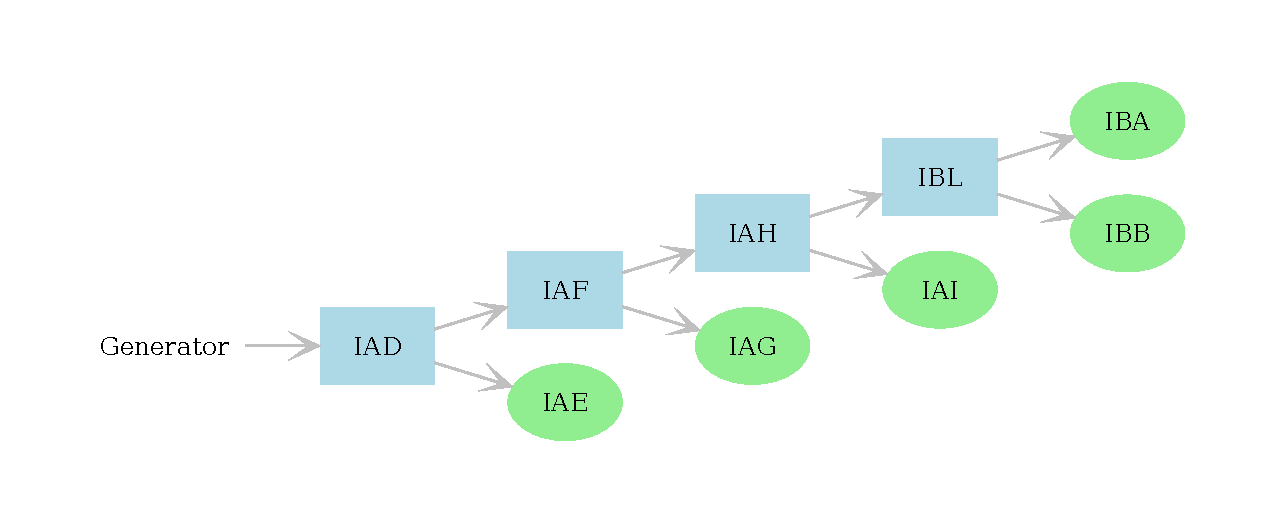
\includegraphics[scale=.7]{subtree.pdf}
  \caption{The simulated subtree.  Airways are represented in light blue, alveoli in light green.}
  \label{fig:subtree}
\end{figure}


% In this project, Chaste has been relied upon generating an anatomical
% surrogate for lungs in premature newborns.

%%% Local Variables:
%%% mode: LaTeX
%%% TeX-master: "../Thesis"
%%% End:

% 3. Anatomical Models
\section{Anatomical Models}
\label{subsec:anatomical_models}

The structure of the internal lung is significantly influenced by the
hierarchical arrangement of the airways, which resemble a fractal
branching tree\cite{suki2011}. The design of this airway tree is
crucial for its function, as the branching pattern affects 
airflow and particle deposition. In modeling the human airway tree, it
is widely accepted that the airways follow an irregular dichotomy
pattern. Unlike regular dichotomy, where each branch splits into two
identical daughter branches, irregular dichotomy results in daughter
branches that can vary significantly in length and diameter.

\vspace{2.25em}

\begin{figure}[H]\centering
  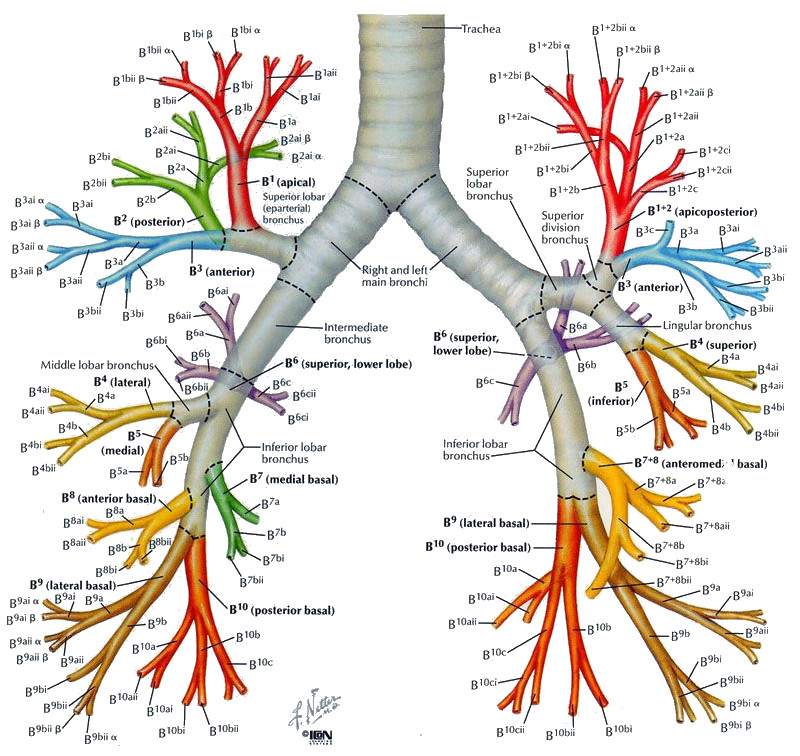
\includegraphics[width=\textwidth]{airway_tree_no_left_best.jpg}
  \caption{Representation of the major airways.}
  \label{fig:airway_tree_anatomical}
\end{figure}

\vspace{2.25em}

% GESTISCI IMMAGINE E TESTO SOTTO
\begin{figure}[H]\centering
  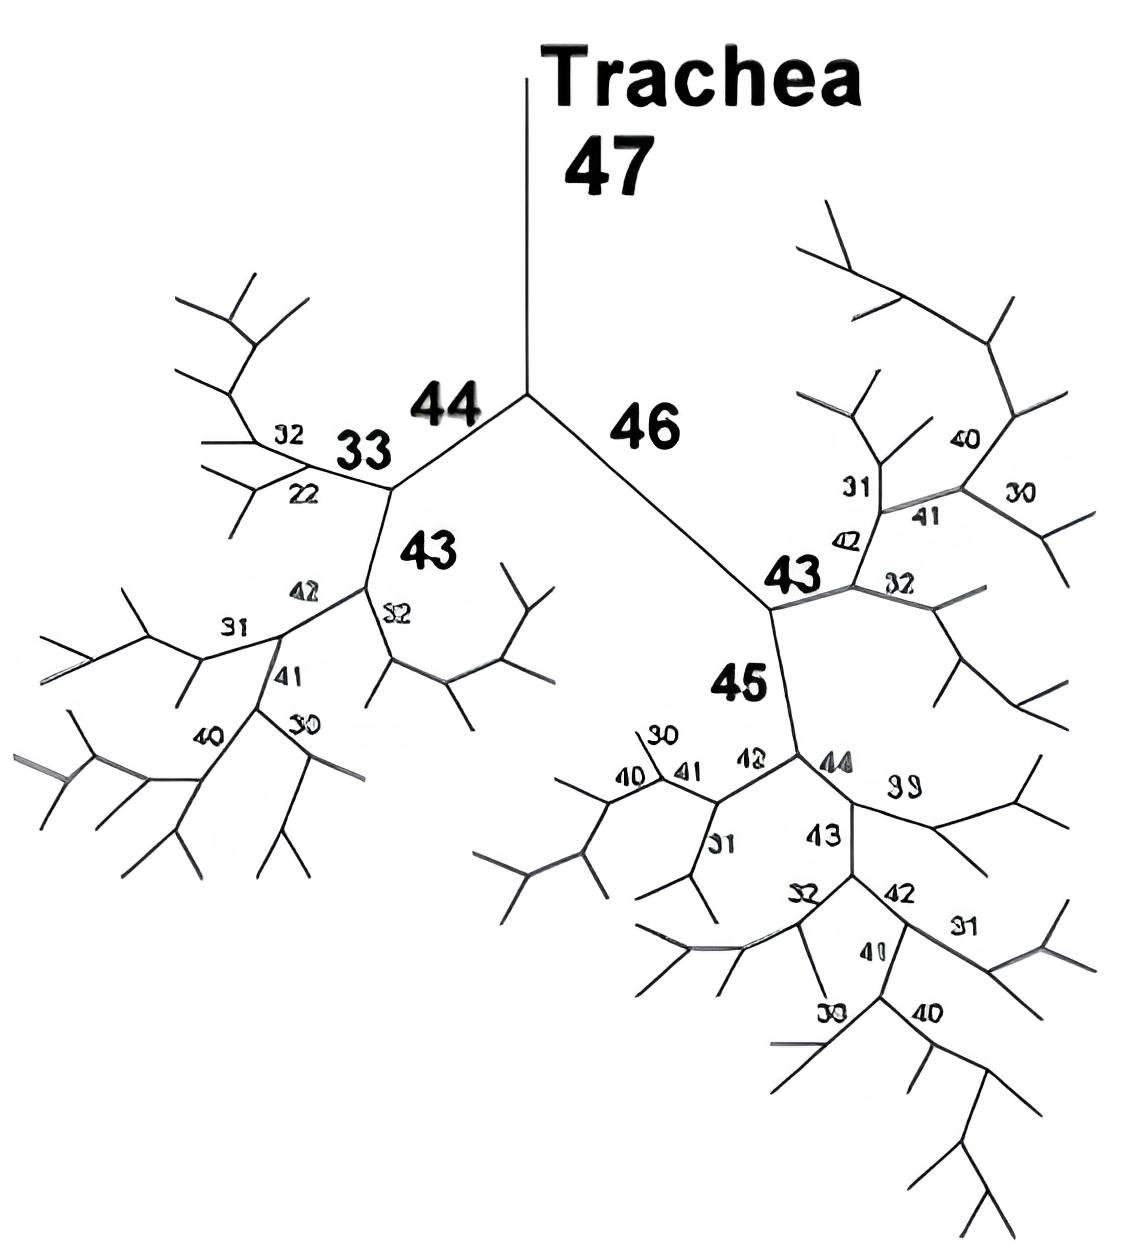
\includegraphics[width=.6\textwidth]{albero_dicotomico_best.png}
  \caption{The dichotomous bronchial tree.}
  \label{fig:albero_dicotomico_anatomical}
\end{figure}

% AGGIUNTA QUESTA MODIFICA, COMPLETARE
% -> spiegato il concetto in inglese.
\Cref{fig:albero_dicotomico_anatomical} serves as a reference for
constructing anatomically coherent adult lungs. In a dichotomous tree,
each airway (excluding the trachea) has a single parent branch and two
daughter branches (excluding the acini).  Asymmetrical bronchial trees
are a specific class presenting uneven splitting: Horsfield orders of
two siblings are different (causing recursion index $\Delta$
to exist, see \cref{fig:airway_impedance}).  Branching angles, lengths, and diameters can vary, thus resulting in different mechanical
properties.

Newborn lungs can be considered as having an analogous structure.

% LEGGERE INTRONORA E TAWHAI, POI CAPIRE COME CITARLI IN QUESTO PUNTO.
% Prima inserisco bene i modelli fregandomene se sono di adulti o
% neonati e poi dico cosa esiste in letteratura.  In questo punto devo inserire anche i parametri Rd, Rl ecc.

3D anatomical models have been generated from CTs by reconstructing
the missing distal airways through
algorithms\cite{tgavalekos2003,tawhai2000}.  Model consistency was
then studied, and its characteristics were compared with histological
measurements\cite{horsfield1987}.  Considering semilogarithmic plots
of the number of branches, lengths, and diameters against Strahler orders,
it is possible to define three important metrics:

\begin{description}
\item $R_{\text{b}}$: The branching ratio. It is defined as the
  antilog of the \emph{absolute value} of the slope of the number of
  branches. It is the factor by which the number of branches increases
  in successive orders \emph{down the tree}.
\item $R_{\text{d}}$: The diameter ratio. It is defined as the antilog
  of the slope of the diameters. It is the factor by which the
  diameter increases in successive orders \emph{up the tree}.
\item $R_{\text{l}}$: The length ratio.  It is defined as the antilog
  of the slope of the lengths.  It is the factor by which the length
  increases in successive orders \emph{up the tree}.
\end{description}


% {\color{red} MANCA QUESTA PARTE. Da tac, .. estratto centerline e
%   ricostruito con diversi algoritmi la parte mancante (Nora, Tawn..).

  % Dei modelli anatomici 3D sono stati realizzati a partire da tac di
  % pazienti, ricostruendo tramite algoritmi la parte mancante di albero
  % (cito Nora e Tawhai perchè modelli
  % diversi\cite{tgavalekos2003,tawhai2000} ).  La consistency del
  % modello è stata studiata confrontando le caratteristiche del modello
  % morfometrico dell'albero con quelle che sono state misurate sui cast
  % ex-vivo, in particolare nora dovrebbe citare cosa sono Rd, Rl ed Rb.
  % Copiare cosa sono questi valori (forse da Nora o Horsfield1987).
%   3D anatomical models have been generated from CTs by reconstructing
%   the missing distal airways through
%   algorithms\cite{tgavalekos2003,tawhai2000}.  Model consistency was
%   then studied, and its characteristics compared with histological
%   measurements.

%   Negli adulti e stato fatto un modello a partire della tac , più la
%   costruzione della parte mancante tramite algoritmi (citazione nora e
%   tawhai). e' stato poi verificato che i parametri morfo (le
%   dimensioni delle vie aeree generate) sono coerenti con quelli
%   ottenuti da misure istologiche. in particolare spiegare rl, rd, ed
%   rb.
% % Questa struttura in \Cref{fig:albero_dicotomico_anatomical} è stata
% usata come riferimento per la costruzione di alberi brochiali
% anatomicamanete coerenti per applicazioni su adulti. 

% PER CITARE NORA: \cite{tgavalekos2003}, PER CITARE TAWHAI
% \cite{tawhai2000}

Instead for infants, there exist models based on the
ovine\cite{al-jumaily2011} and canine\cite{herrmann2016} anatomy.

Mathematical models developed for adult lungs cannot simply be scaled
down to fit the lungs of newborns. Newborn lungs are not
simply one miniature version of adult lungs, but they present
significant differences in terms of bronchial branch proportions,
constituents of the airways\cite{merkus1996}, morphometric
characteristics ($R_{\text{d}}$, $R_{\text{l}}$,
$R_{\text{b}}$)\cite{horsfield1987} and composition\cite{hislop1989}.

%% Citare qui i riferimenti che ha fatto chiara nella call del 21.06
\textcite{mani2020} considered an adult lung model linearly scaled to
match newborn anatomical features.  The advantage of this approach is
that it respects the dimensions of the trachea and bronchioles. It doesn't
guarantee that the morphometric characteristics of the entire airway
tree are respected.  In this work, a few airway generation
parameters can be adapted, to better approximate
the target morphometric characteristics.

%%% Local Variables:
%%% mode: LaTeX
%%% TeX-master: "../Thesis"
%%% End:

% 4. Mechanical Model of Airways and Acini
\section{Mechanical Model of Airways and Acini}

% (cambiare `acini`) (paper in chat Lutchen). (no zsoft e
% cartilagine)

% Scrivere in breve la struttura circuitale che poi implemento
% (copia).

% La struttura circuitale è descritta in lutchen1997 in marrone.

The adult airway can be likened to a transmission line (see
\cref{fig:airway_impedance}), with resistors, capacitors, and
inductors having constant values.  These components form a circuit as
illustrated.  Moreover, tissues properties ($Z_{\text{w}}$) are
incorporated.  \Cref{fig:airway_impedance,fig:acinus_impedance} show
modules connected according to the structure of the newborn airway,
which is comparable to that depicted in
\cref{fig:albero_dicotomico_anatomical}.  $Z(n)$ represents the parent
branch as a function of the Horsfield order, while $Z(n-1)$ and
$Z(n-1-\Delta)$ denote the two daughters branches.  $Z(2)$ represents
the terminal airway.  Each airway has a parent branch (excluding the
trachea) and two daughter branches (excluding the acini).

% L'equivalente elettrico delle proprietà dei tessuti è stato modificato
% per poter testare l'impatto delle modifiche fisiologiche durante il
% processo di aereazione.

The electrical equivalent of tissue properties is modified to test
the physiological change impact on the aeration process.

% Inoltre, il liquido fetale è incomprimibile, l'aria invece non lo è,
% comportando la presenza di un elemento aggiuntivo nell'equivalente
% elettrico dell'aria, in quanto la compressibilità del gas è
% modellizzata attraverso una capacità. In aggiunta, bisogna tener conto
% del collasso delle vie aeree, perché durante il processo di aerazione
% si crea un'interfaccia aria-liquido, che a sua volta dà origine a una
% tensione superficiale, la quale deve essere superata per permettere lo
% spostamento del fluido nell'albero bronchiale.  Una volta superata, i
% diametri si possono ingrandire facendo aumentare il volume polmonare.

The air-fluid interface modulates the values of resistances and
inductances in both the module types.

Moreover, this fluid is incompressible, whereas air is not. This
introduces an additional element in the electrical equivalent of air,
as the compressibility of the gas is modeled through a
capacitance.

% Additionally, it is necessary to consider the collapse of
% the airways.

During the aeration process, an air-liquid interface is created, which
in turn, generates surface tension that must be overcome to allow fluid
movement within the bronchial tree. Once this surface tension is
overcome, the diameters can expand, leading to an increase in lung
volume.

\textcite{lutchen1997} have developed a mechanical lung model in
frequency-domain, describing airways and acini modules as displayed
in \cref{fig:airway_impedance} and \cref{fig:acinus_impedance},
respectively.

\vspace{2.25em}

% Circuiti copiato da lutchen1997. 
\begin{figure}[H]\centering
  \begin{circuitikz}[scale=.9]
    % Circuit
    %% Main branch
    %%% Input Node
    \draw (1.5,0)
    node[ocirc] (circuit_IN) {}
    to[short, ] ++(1,0) coordinate(R_IN)
    ;
    
    %% Main branch
    \draw (R_IN)
    to[short] ++(.5,0)
    to[resistor, l=$R(n) / 2$] ++(1,0)
    to[inductor, l=$I(n) / 2$] ++(3,0) coordinate (C_g_IN)
    to[short] ++(1.5,0) coordinate (SW_IN)
    to[resistor, l=$R(n) / 2$] ++(3,0)
    to[inductor, l=$I(n) / 2$] ++(1,0)
    to[short, -*] ++(1,0) coordinate(circuit_OUT)
    ;

    %%% C_g branch
    \draw (C_g_IN)
    to[polar capacitor, invert, l_=$C_{\text{g}}(n)$, *-] ++(0,-3.5)
    node[ground]{} ++(0,0)
    ;

    %%% Zw branch
    \draw (SW_IN)
    to[twoport, t={$Z_{w}(n)$},bipoles/twoport/height=1.2, *-] ++(0, -3.5)
    node[ground]{} ++(0,0)
    ;

    \draw (circuit_OUT)
    -- ++(0, .5)
    to ++(1.88,0)
    node[draw, anchor=west, thick] {$Z(n-1)$};
    
    \draw (circuit_OUT)
    -- ++(0, -.5)
    to ++(1,0)
    node[draw, anchor=west, thick] {$Z(n-1-\Delta$)};

    % Nodes
    %% IN
    \draw[->, >=stealth, thick] (0,0) -- (circuit_IN) node[midway, above] {Z(n)};
  \end{circuitikz}
  \caption{Impedance ($Z$) of a given order ($n$) of a single airway
    generation is calculated via an acoustic transmission line
    analysis, which accounts for shunting into gas compression in the
    tube ($C_{\text{g}}(n)$) and into nonrigid airway walls
    ($Z_{\text{w}}$)\cite{lutchen1997}.}
  \label{fig:airway_impedance}

\end{figure}

%%% Local Variables:
%%% mode: LaTeX
%%% TeX-master: "../Thesis"
%%% End:


\vspace{2.25em}

\begin{figure}[H]\centering
  \begin{circuitikz}[scale=1.3]
    % Circuit
    %% Main branch
    %%% Input Node
    \draw (1.5,0)
    node[ocirc] (circuit_IN) {}
    to[short, ] ++(1,0) coordinate(Z_IN)
    to[twoport, bipoles/twoport/width=1.0, t=$Z(2)$] ++(2,0) coordinate(C_g_IN)
    ;
    
    %% Main branch
    % \draw (Z_IN)
    % to[twoport, t=$Z_{2}$] ++(2,0) coordinate(C_g_IN)
    % ;

    %%% C_g branch
    \draw (C_g_IN)
    to[polar capacitor, invert, l_=$C_{\text{g}}(n)$, *-] ++(0,-3.5)
    node[ground]{} ++(0,0)
    ;

    %%% Zw branch
    \draw (C_g_IN)
    to[inductor, l=$I_{\text{t,i}}$] ++(2, 0)
    to[twoport, t={$\dfrac{G - j\cdot H}{\omega^\alpha}$},bipoles/twoport/width=2.0, bipoles/twoport/height=1.2] ++(3, 0)
    to[short] ++(0, -3.5)
    node[ground]{} ++(0,0)
    ;

  \end{circuitikz}
  \caption{An alveolar-tissue element is attached to the terminal
    airways in the tree. There is gas compression corresponding to
    volume of the acinus ($C_{\text{g}}$) and the tissue element is
    viscoelastic containing a tissue damping ($G$) coupled to
    elastance ($H$) to ensure a constant tissue hysteresis. $j$:
    imaginary unit, $I_{\text{t,i}}$: tissue
    inertance\cite{lutchen1997}.}
  \label{fig:acinus_impedance}

\end{figure}

%%% Local Variables:
%%% mode: LaTeX
%%% TeX-master: "../Thesis"
%%% End:


In this thesis, as well as in \textcite{mani2020}, a mechanical model
is defined in time-domain starting from the modules described in this
section and properly adapted.

% AGGIUNTA MODIFICA, COMPLETARE
% -> la parte sul fluido è stata inserita sopra
% -> la parte del diodo è stata inserita sotto.

% In questo punto devo inserire la spiegazione del modello in cui si
% inserisce anche il diodo, oltre al liquido. proprio perché mani2020
% è stata la prima ad inserirlo.

% liquido .. diodo

Capillary pressure is due to the air-fluid interface in the airway tree.
It was considered and modeled as a diode component: opening
threshold voltage corresponds to the aforementioned capillary
pressure for a generic airway.

% Da spostare in implementation? 
A first implementation has been performed on the «CADENCE» platform.  This
has the advantage of parallelism and speed.  There are also some
drawbacks to this approach: this framework is designed to simulate
standard electrical components and it is not well-suited to develop
time- and current integral-dependent components.  Furthermore, the license
is proprietary and machine-specific.  This limits the accessibility
of the model design process.

% Posso dire che l'alveolo è stato modificato (vedi Veneroni2024) a
% partire dall'alveolo mostrato da lutchen1997 perché non risolvibile
% nel dominio del tempo.

%%% Local Variables:
%%% mode: LaTeX
%%% TeX-master: "../Thesis"
%%% End:

% 5. Model Development
%   5.1. Anatomical Model
%     5.1.1. CT Image Processing: Lung Segmentation, Centreline and Radii Extraction
%     5.1.2. Algorithmic Generation of the Distal Airway Centreline
%   5.2. Mechanical Model
%     5.2.1. Programming Language --- Model Designing & Instantiating
%     5.2.1.1  Callbacks' Role in State Variables Discontinuity Handling
%     5.2.3. Model Testing

\section{Model Development}
\label{sec:model_development}

% Mettere enfasi sulla ricerca dei metodi perché Julia e non altro.

% Visione d'insieme (diagramma con flusso dell'informazione, data
% pipeline). Questo diagramma mostra a partire dagli input che ho
% avuto (TC) tutto l'iter del dato.

% Qui ha detto poi Chiara che conviene inserire delle informazioni
% riguardanti i modelli matematici utilizzati.

This chapter describes the methods used to develop an open-source, 3D
morphometric neonatal lung model that allows simulations of lung
aeration at birth.

An anatomically coherent 3D lung model is combined with a mechanical
model of the airways and acini, able to simulate changes in the
mechanical properties of the airways when the lung fluid is replaced
by air entering the lungs.

The sequence for model development is reported in
\cref{fig:data_pipeline}. We extracted a 3D surface mesh of lung lobes
and airway centrelines from a lung CT of a newborn. We implemented a
statistical method, previously described for adult lung models, able
to generate distal airways that were not visible on the CT. We adapted
the method for the newborn lung.

We implemented a mechanical model of the airways and acini whose
parameters are dependent on the airway's lengths and diameters and the
presence of fetal fluid, fetal fluid-air interface, or air in the
airway. We exploited an open-source solver for differential equations
to simulate the network.

\begin{figure}[]\centering
  % todo: modificare l'immagine sopra ad "anatomical surrogate generation" con uno screen di ParaView.
% todo: aggiungere immagini sopra al branch del modello meccanico.

\begin{figure}[H]\centering
  \begin{tikzpicture}[node distance=3cm]
    % Nodes
    %% Chaste & Morphometric Model
    \node (ct_acquisition)           [startstop] {CT\\Acquisition};
    \node (img_ct_acquisition)       [image, above of=ct_acquisition, yshift=-1.0cm]                   {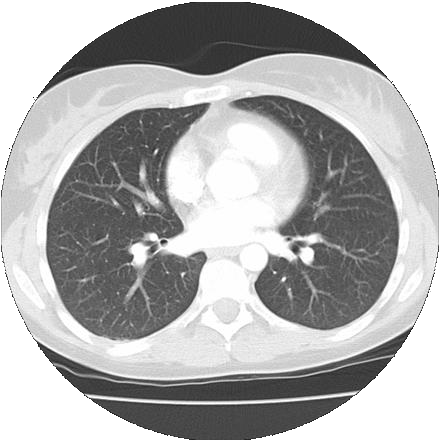
\includegraphics[width=2.0cm]{ct_acquisition.png}};
    %%% Upper branch
    \node (lobes_segmentation)       [process, right of=ct_acquisition, xshift=3.25cm, yshift=+2cm]    {Lobes\\segmentation};
    %%% Lower branch
    \node (img_lobes_segmentation)   [image, above of=lobes_segmentation, xshift=-.1cm, yshift=-1.2cm] {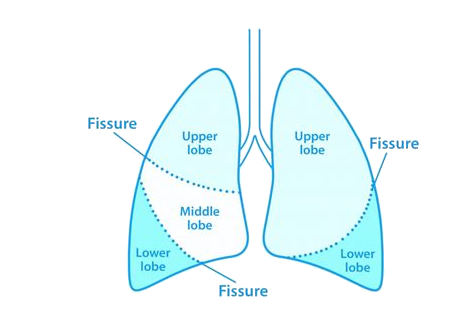
\includegraphics[width=3.5cm]{lobes_segmentation.png}};
    \node (airways_segmentation)     [process, below of=lobes_segmentation, xshift=-2cm, yshift=-1cm]  {Airways\\segmentation};
    \node (img_airways_segmentation) [image, above of=airways_segmentation, xshift=2cm, yshift=-1cm]   {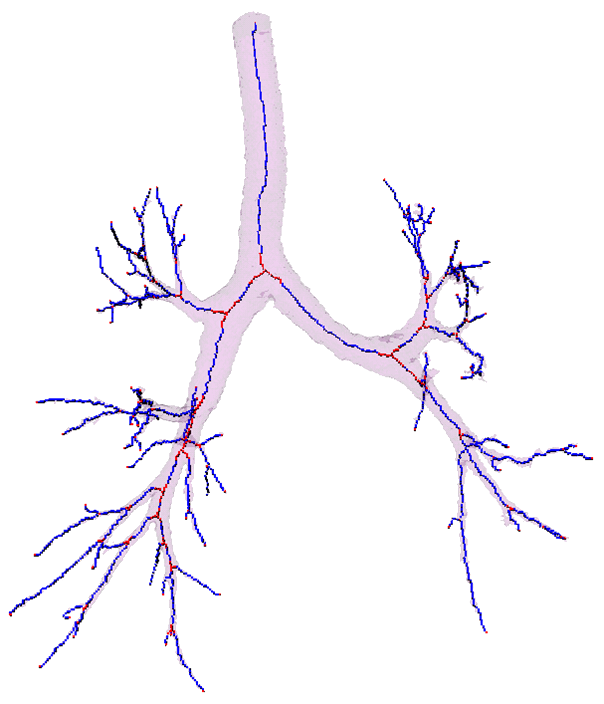
\includegraphics[height=2.5cm]{airways_segmentation.png}};
    \node (centerline_extraction)    [process, below of=lobes_segmentation, xshift=+2cm, yshift=-1cm]  {Centerline\\extraction};
    \node (surrogate_generation)     [process, right of=ct_acquisition, xshift=9.5cm]                  {Anatomical surrogate\\generation};
    \node (img_surrogate_generation) [image, above of=surrogate_generation, yshift=-.5cm]              {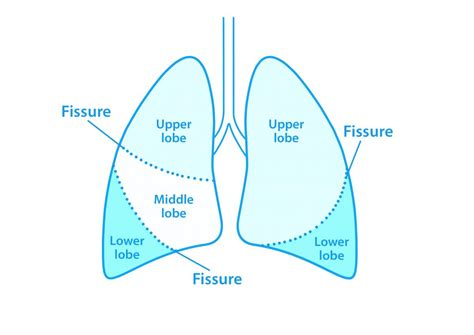
\includegraphics[width=3.5cm]{lobes_segmentation.jpg}};
    %% Julia & Mechanical Model
    \node (parameters_update)        [process, below of=ct_acquisition, yshift=-3cm]                   {Lungs parameters\\update};
    \node (model_instantiation)      [process, right of=parameters_update, xshift=1cm]                 {Mechanical model\\instantiation};
    \node (DAE_solution)             [process, right of=model_instantiation, xshift=1cm]               {DAE System\\solution};
    \node (simulations)              [startstop, right of=DAE_solution, xshift=+1cm]                   {Mechanical Simulations};

    % Arrows
    \draw [arrow] (ct_acquisition.east)                              -- ++(.5,0) coordinate(tmp)     |- (airways_segmentation.west);
    \draw [arrow] (airways_segmentation)                             -- (centerline_extraction);
    \draw [arrow] (centerline_extraction.east)                       -- ++(.5,0) coordinate(tmp1)    |- (surrogate_generation.west);
    \draw [arrow] (model_instantiation)                              -- (DAE_solution);
    \draw [arrow] (DAE_solution)                                     -- (simulations);
    \draw [arrow] (tmp)                                              |-   (lobes_segmentation.west);
    \draw [arrow] (lobes_segmentation)                               --   (tmp1|-lobes_segmentation) |- (surrogate_generation.west);
    \draw [dashed, thick, ->,>=stealth] (surrogate_generation.south) -- ++(0,-3.5)                   -| (parameters_update.north);
    \draw [arrow] (parameters_update)                                -- (model_instantiation);

    % Frame around a part of the flowchart
    \begin{pgfonlayer}{background}
      \node[rounded corners=3mm,
      draw=blue,
      thick, dashed,
      fit=(airways_segmentation)(centerline_extraction)(img_lobes_segmentation)(img_surrogate_generation),
      fill=cyan!5,
      inner sep=7pt,
      label={[anchor=north]below:\textsc{\textcolor{blue}{Chaste \& Morphometric model}}}] {};
    \end{pgfonlayer}
    \begin{pgfonlayer}{background}
      \node[rounded corners=3mm,
      draw=red,
      thick, dashed,
      fit=(parameters_update)(model_instantiation)(DAE_solution),
      fill=magenta!5,
      inner sep=7pt,
      label={[anchor=north]below:\textsc{\textcolor{red}{Julia Programming Language \& Mechanical model}}}] {};
    \end{pgfonlayer}
  \end{tikzpicture}
  \caption{Data pipeline.  The process begins with a
    \emph{patient-specific image} (i.e. CT) of a premature newborn.
    The extracted data, comprising \emph{two segmentations}, are then
    processed to obtain an anatomical surrogate of the airway tree.
    This is necessary due to scanner resolution not allowing for the
    discrimination and localization of small branches.  From the
    resulting morphometric model, the \emph{mechanical parameters} can
    be derived, which are essential for generating an accurate
    simulation model.  Finally, a numerical solver for differential
    equations provides the final output.}
    \label{fig:data_pipeline}
\end{figure}

%%% Local Variables:
%%% mode: LaTeX
%%% TeX-master: "../Thesis"
%%% End:

  % \begin{figure}[h!]
  \centering
  \scalebox{.75}{
    \begin{tikzpicture}[]
      % Nodes
      %% Chaste & Morphometric Model
      \node (ct_acquisition)           [startstop] {CT Acquisition};
      %%% Upper branch
      \node (lobes_segmentation)       [process, right of=ct_acquisition, xshift=8.25cm, yshift=+1cm]      {Lobes segmentation};
      \node (airways_segmentation)     [process, below of=lobes_segmentation, xshift=-2.5cm, yshift=-1cm]  {Airways segmentation};
      \node (centreline_extraction)    [process, below of=lobes_segmentation, xshift=+2.5cm, yshift=-1cm]  {Centreline extraction};
      \node (anatomical_generation)    [process, minimum width=5cm, text width=5cm, right of=ct_acquisition, xshift=16.5cm]                  {Algorithmic Generation of Distal Airway Centrelines};
      %% Julia & Mechanical Model
      \node (airways_model)            [startstop, below of=ct_acquisition, yshift=-5cm]               {Airways model};
      \node (acini_model)              [startstop, below of=airways_model, yshift=-1cm]                  {Acini model};
      \node (model_instantiation)      [process, below of=airways_segmentation, yshift=-5cm]                     {Mechanical model instantiation};
      \node (DAE_solution)             [process, below of=centreline_extraction, yshift=-5cm]               {DAE System solution};
      \node (tracheal_pressure)        [startstop, above of=DAE_solution, yshift=2.5cm]                      {Tracheal pressure waveform};
      \node (simulations)              [startstop, below of=anatomical_generation, yshift=-6cm]                   {Simulations results};
      \node (phi_length)               [startstop, minimum width=5cm, text width=4.5cm, above of=model_instantiation, yshift=2.5cm]                 {Diameters, length, father airway of each airway};
      
      
      % % Arrows
      \draw [arrow] (ct_acquisition.east)                              -- ++(1.5,0) coordinate(tmp)     |- (airways_segmentation.west);
      \draw [arrow] (airways_segmentation)                             -- (centreline_extraction);
      \draw [arrow] (centreline_extraction.east)                       -- ++(.5,0) coordinate(tmp1)    |- (anatomical_generation.west);
      \draw [arrow] (model_instantiation)                              -- (DAE_solution);
      \draw [arrow] (DAE_solution)                                     -- (simulations);
      \draw [arrow] (tmp)                                              |-   (lobes_segmentation.west);
      \draw [arrow] (lobes_segmentation)                               --   (tmp1|-lobes_segmentation) |- (anatomical_generation.west);
      \draw [arrow] (phi_length.south)  -- (model_instantiation.north);
      \draw [arrow] (acini_model.east) -- ++(1.5,0)  |- (model_instantiation.west);
      \draw [arrow] (tracheal_pressure.south) -- (DAE_solution.north);
      \draw [arrow] (airways_model.east) -- ++(1.5,0)  |- (model_instantiation.west);
      \draw [dashed, thick, ->,>=stealth] (12.5,-1.775) -- ++(0,-.50)                   -| (phi_length.north);

      
      % % Frame around a part of the flowchart
      \begin{pgfonlayer}{background}
        \node[rounded corners=3mm,
        draw=blue,
        thick, dashed,
        % fit=(airways_segmentation)(centreline_extraction)(img_lobes_segmentation)(img_anatomical_generation),
        fit=(airways_segmentation)(centreline_extraction)(lobes_segmentation)(anatomical_generation),
        fill=cyan!5,
        inner sep=7pt,
        label={[anchor=south]above:\textsc{\textcolor{blue}{Morphometric model}}}] {};
      \end{pgfonlayer}
      \begin{pgfonlayer}{background}
        \node[rounded corners=3mm,
        draw=red,
        thick, dashed,
        fit=(airways_model)(acini_model)(model_instantiation)(DAE_solution),
        fill=magenta!5,
        inner sep=7pt,
        label={[anchor=north]below:\textsc{\textcolor{red}{Mechanical model}}}] {};
      \end{pgfonlayer}
    \end{tikzpicture}
  }
  \caption{Data pipeline.  The process begins with a
    \emph{patient-specific image} (i.e. CT) of a premature newborn.
    The extracted data, comprising \emph{two segmentations}, are then
    processed to obtain an anatomical surrogate of the airway tree.
    This is necessary due to scanner resolution not allowing for the
    discrimination and localization of small branches.  From the
    resulting morphometric model, the \emph{mechanical parameters} can
    be derived, which are essential for generating an accurate
    simulation model.  Finally, a numerical solver for differential
    equations provides the final output.}
  \label{fig:data_pipeline}
\end{figure}

%%% Local Variables:
%%% mode: LaTeX
%%% TeX-master: "../Thesis"
%%% End:

  \caption{Data pipeline.  The process begins with a
    \emph{patient-specific image} (i.e. CT) of a premature newborn.
    The extracted data, comprising \emph{two segmentations}, are then
    processed to obtain an anatomical surrogate of the airway tree.
    This is necessary because scanner resolution does not allow for the
    discrimination and localization of small branches.  From the
    resulting morphometric model, the \emph{mechanical parameters} can
    be derived, which are essential for generating an accurate
    simulation model.  Finally, a numerical solver for differential
    equations provides the final output.}
  \label{fig:data_pipeline}
\end{figure}
  
%   2.2. Morphometric model
\subsection{Anatomical Model}
\label{subsec:airway_development}
% Per Chiara: Inserisco definizione di modello morfometrico?
Morphology generation process is required as it is not possible to
obtain high generations (aka small airways) using standard
high-resolution CT\cite{bordas2015}.

There are different open-source platforms available for generating
adult morphometric models.  In particular:

\begin{enumerate}
\item AVATree (Windows-only)
\item Chaste (cross-platform) library
\end{enumerate}

Due to problems related to «AVATree» source code compilation for
Windows with «Visual Studio», Chaste library is selected for this
project.

Chaste is a C++ open-source (BSD licensed) library developed by Oxford
University.  It has multiple use cases across various biomedical
fields, with an emphasis on cardiac electrophysiology and cancer
development\cite{mirams2013}.  It can be integrated into a C++ program
or used via «User Project» (i.e. \texttt{ctest}).  Specifically, the
``AirwayGenerationTutorial'' is considered as a first code base and
properly adapted to match newborn
parameters\cite{airwaygeneration2024}.

The required input consists of two pieces of information:
\begin{itemize}
\item A \emph{mesh of centreline points}.  This mesh is provided in
  TetGen format, comprising ``airways.node'' and ``airways.edge''
  files. The first file lists centreline point coordinates,
  respective sampled airways radius, and a boolean value to indicate if
  the point is generative. The second one contains all the connections
  between pairs of points.
\item Four (or five) \emph{lobes segmentations} in STL format.  These
  segmentations are necessary as they physically impose a limit on the
  growth algorithm.
\end{itemize}

\subsubsection{CT Image Processing: Lung Segmentation, Centreline and
  Radii Extraction}
\label{subsubsec:ct_centreline_radii_extraction}
% todo: Devo chiedere bene a Francesca come sono stati estratti i
% raggi.

«3D Slicer» is an open-source software used for CT image processing.
Two extensions are installed:

\begin{description}
\item «\emph{Chest\_imaging\_platform}»: This extension enables
  semi-automatic segmentation of major airways from a single fiducial
  point.  It can also extract adult lobes using three fiducial points
  per lung fissure. However, in our case, the fissures are not
  visible, necessitating manual intervention.
\item «\emph{SlicerVMTK}»: This extension is used for extracting
  centreline points.
\end{description}

\subsubsection{Algorithmic Generation of the Distal Airway Centreline}
\label{subsubsec:statistical_generation}

The Chaste User Project reads the input files (see
\cref{subsec:airway_development}), and begins growing the anatomical
surrogate from the points labeled as «generative».  The algorithm
operating under the hood is a modified version\cite{bordas2015} of the
one described by \textcite{tawhai2000}.  The generated output is
available in various formats:

\begin{itemize}
\item VTU: Unstructured Grid (base64 encoded) format used by VTK
  library.  It can be displayed by ParaView, an open-source viewer.
\item node and edge: TetGen format.  Such files are better suited for
  further processing.
\end{itemize}

% bordas2015 parla anche di come vengono generate le vie aeree e come
% vengono assegnati i diametri.

% AGGIUNTA MODIFICA, COMPLETARE
% prima. -> SPOSTO LA FRASE IN SOTTOSEZIONE PARENTE.
This process is required as it is not possible to obtain high
generations (aka small airways) using standard high-resolution
CT\cite{bordas2015}.

% {1} va spiegato qui, poi descriviamo l'algoritmo
A uniform grid of seed points is created within each segmented lobar
surface. Seed points approximately correspond to terminal bronchioles.
The spacing of the seed point grid is set so that the mean volume around
each of such points corresponds to the acinar volume (for adults being
$187\text{mm}^3$, for 5-weeks old newborns $5.3\text{mm}^3$).
% AGGIUNTA MODIFICA, COMPLETARE
% -> AGGIUNTO VALORE PER NEONATO 5W (da dove è stato recuperato?)

The starting points of the algorithm are the distal ends of the
segmented airway centrelines.  These points are also referred to as
growth apices.

An \emph{adaptive threshold} on the distance between the seed points
and growth apices is required to prevent spurious long airways from being
generated in the last few generations.  \Cref{eq:airway_threshold}
describes such threshold:

\begin{equation}
  T = \max(V_{\text{b}} - n\cdot D_{\text{l}}, 5\text{mm})
  \label{eq:airway_threshold}
\end{equation}

Where:
\begin{description}
\item $V_{\text{b}}$ is the diagonal size of the bounding box of the lobe being
  generated into.
\item $D_{\text{l}} (= {V_{\text{b}}/{N}})$ is the distance limit.
\item $N$ is the maximum number of generations.
\item $n$ is the current generation number.
\end{description}

With these definitions, the \textbf{growing algorithm} is described as
such:

\begin{enumerate}
\item \emph{Each seed point is associated with the closest growth apex
    within its lobe}.  The seed point having a distance to a
  growth apex greater than the aforementioned adaptive threshold is
  not associated with that distal end.  If all distal ends are further
  than the threshold from the seed point, the seed point remains
  unlabeled.
\item \emph{Calculation of the centroid of points assigned to each
    distal branch.}
\item \emph{The plane defined by the centroid and the parent branch is
    used to split the points into two unequal sets.}
\item \emph{Centroids of each of the new point sets are calculated.}
\item \emph{For each set of points a new airway is generated} starting
  at the distal end and extending 40\% of the distance towards the
  centroid of the point set.  This value is arbitrarily chosen for adults but kept for
  newborns.  It must be optimized in future developments.
\item \emph{Generated branches are checked to determine whether it is
    terminal}.  Branches whose length is less than $2\text{mm}$ (for
  adults, to be changed with $.12\text{mm}$ for newborns) are
  considered terminal.  Also, branches whose point set contains just a
  single point are considered terminal points.  For all
  terminal branches, their associated seed point is discarded from the
  global set.
\item \emph{Iterate} until no seed point is available.
\end{enumerate}

% DA DOVE VIENE FUORI .12 MM?
% sarebbe interessante capire come cambiare quel 2mm.

\textbf{Diameters} are computed by means of \cref{eq:lumen_diameter}.

\begin{equation}
  \log D(x) = (x - N)\log(R_{\text{d}} H) + \log(D_{\text{N}})
  \label{eq:lumen_diameter}
\end{equation}

Where:
\begin{description}
\item $D$ is the airway diameter.
\item $x$ is the current Horsfield order.
\item $N$ is the maximum Horsfield order.
\item $D_{\text{N}}$ is the maximum diameter.
\item $R_{\text{d}} H$ is the anti-log of the slope of airway diameter
  plotted against Horsfield order and is set to 1.15 for adults, 1.33
  for 5w newborns\cite[][Tab. 2]{horsfield1987}.  This parameter in
  the code is named ``DiameterRatio''.
\end{description}
  
\subsection{Mechanical Model}
\label{subsec:simulator_development}

In order to perform simulation it is required to use an efficient
differential equation solver.

«\texttt{DifferentialEquations.jl}» wraps all available solvers (even
C and FORTRAN ones) and it is very efficient
\cite{diffeqdocs2024,rackauckas2017}.

Julia is a free, open-source (MIT licensed), fast, scientific and
numerical computing-oriented programming language.  Its computational
efficiency is comparable to statically typed languages like C
or FORTRAN.  Moreover, its high-level code expressiveness rivals that of
languages like Python, R, and MATLAB\cite{juliadocs2024}.

Two key features, inspired by the \emph{Lisp Language}, are
highlighted here.

\begin{description}
\item \emph{Metaprogramming}: Code is treated as any other Julia data
  structure and, thus can be dynamically generated and manipulated at
  runtime.
\item \emph{Macros}: They help instantiate the generated code in the
  body of a program.
\end{description}

Their importance is closely tied to the concept of Domain-Specific
Languages (aka DSLs).  These dialects are composed of abstractions
that can be properly exploited to solve particular problems
(e.g. modeling complex systems, solving differential equations).

Julia REPL has a built-in package manager (i.e. «\texttt{Pkg.jl}»)
used for managing project dependencies and ensuring the
\emph{repeatability} of computational setups.  This is achieved by
saving the required package names and commits into `Project.toml' and
`Manifest.toml' files.

\subsubsection{Programming Language --- Model Designing \& Instantiating}
\label{subsubsec:modelingtoolkit}

«\texttt{ModelingToolkit.jl}» encompasses all the tools necessary for
model design.  This Julia package is equation-driven, requiring each
system to be described by Differential-Algebraic Equations (i.e. DAEs)
for subsequent solving\cite{ma2021}. Its built-in DSL optimizes every
stage of modeling, from prototyping components to instantiating the
complete system.

An acausal paradigm can be adopted, allowing users to reason in terms
of \emph{components}\cite{mtkdocs2024}. This modularity facilitates
system extensibility compared to the causal approach, where the entire
system of Differential-Algebraic Equations must be considered and
manually simplified\cite{ma2024}.

In particular, the usage of \jlinl{@mtkmodel} macro enables
hierarchical generation of building blocks recurring in the
highest-order model (i.e. «Lungs»).  Here is how information is
structured within \jlinl{@mtkmodel} macro.

\begin{jllisting}[label=@mtkmodel, caption={\jlinl{@mtkmodel}: a macro for systems prototyping.}]
  @mtkmodel <name_of_model> begin
      @parameters begin
          # (Optional) Some constant (e.g. Resistance, Capacitance) ...
      end
      @components begin
          # (Optional) Some dependency system (e.g. Resistor, Capacitor) ...
      end
      @variables begin
          # (Optional) Internal variables ...
      end
      @equations begin
          # Differential Algebraic Equations describing the model's behavior.
      end
      @continuous_events begin
          # (Optional) Some callback function ...
      end
  end
\end{jllisting}

Replicating the behavior of electrical components using this language
is straightforward, once you are familiar with the syntax and
understand the Differential-Algebraic Equations that represent their
characteristics.  Each generated system can then be composed into more
complex ones, using the internal \jlinl{@components} macro, thereby
implementing the hierarchical structure mentioned earlier.

After describing the highest-order system, the Julia compiler requires its
instantiation before any simulation can be performed.  This is
accomplished using \jlinl{@mtkbuild} macro, which minimizes the number
of equations that need to be solved.

Code modularity is directly reflected in the electrical equivalent
circuit.  Specifically, by encapsulating systems with the internal
\jlinl{@components} macro, it becomes possible to generate models of
increasing complexity.  This approach enables a clear separation
between components that belong to different hierarchical levels and
facilitates compartmentalization during the model design phase.

\vspace{.5em}

{\normalsize\textbf{Callbacks' Role in State Variables
      Discontinuity Handling}} Not all characteristics of electrical
components can be defined solely by DAEs.  Voltages or currents may
suddenly change, triggered by a circuit event.  In such cases,
\emph{continuous callback functions} can be employed to appropriately
alter the value of state variables.  These callbacks consist of two
functions:
\begin{itemize}
\item \texttt{condition}: Specifies the event to be tested.
\item \texttt{affect}: Defines how the state variable(s) should be
  changed.
\end{itemize}

The component-based approach allows for the definition of callbacks
directly within the (sub)system being modeled.

% Example of usage?

\subsubsection{Airways and Acini Models}
\label{subsubsec:blocks_description}


% 1. È necessario indicare la notazione utilizzata nelle formule?
% 2. Su cosa devo concentrarmi nella descrizione? Devo mostrare
% codice?

The following blocks are listed in a bottom-up order (from lowest to
highest).

\begin{enumerate}
\item \textbf{Mathematical and Electrical Components}.  The simplest
  blocks are derived from the standard library of components (aka
  «\texttt{ModelingToolkitStandardLibrary.jl}»), while integral-dependent
  ones rely on a modified mathematical block to manage both current
  integration and its timing correctly.  Their behavior varies based
  on the neonatal pulmonary fluid interface.
  \begin{description}
  \item \emph{Current Integrator}: it computes the current integral
    and manages integration timing through a Callback function
    (see the former Callbacks Section).
  \item \emph{Current Integral-Dependent Inductor}: It takes the
    current integral value from the Current Integrator and computes the
    inductance value according to this formula
    $L(t) = L_{\text{a}} + L_{\text{b}}\cdot \left(1 - \dfrac{\int
        {i(t) dt}}{V_{\text{FRC}}}\right)$, where $L_{\text{a}}$ is
    the inductance when air-filled, $L_{\text{b}}$ is the difference
    between liquid and air inductances, $V_{\text{FRC}}$ is the volume
    at FRC (i.e., Functional Residual Capacity).
  \item \emph{Current Integral-Dependent Resistor}: It takes the
    current integral value from the Current Integrator and computes the
    resistance value according to this formula
    $R(t) = R_{\text{a}} + R_{\text{b}}\cdot \left(1 - \dfrac{\int
        {i(t) dt}}{V_{\text{FRC}}}\right)$, where $R_{\text{a}}$ is
    the resistance when air-filled, $R_{\text{b}}$ is the difference
    between liquid and air resistances, $V_{\text{FRC}}$ is the volume
    at FRC.
  \item \emph{Diode}: It is modeled as a voltage generator whose
    activation state is dependent on the fill-up states of the
    previous and the current module ($\text{trigger}_{\text{in}}$ and
    $\text{trigger}_{\text{out}}$, respectively). Its behavior is
    summarized by the following formula:
    $\Delta V = \text{trigger}_{\text{in}} \cdot (1 -
    \text{trigger}_{\text{out}}) \cdot V_{\text{in,th}}$, where
    $\Delta V$ is the voltage drop across the component and
    $V_{\text{in,th}}$ is the diode voltage threshold. This is a
    custom component and it does not come as part of the standard
    library.
  \item \emph{Inductor}: Constant component.
  \item \emph{Resistor}: Constant component.
  \end{description}
\item \textbf{Modules}.  Obtained by connecting the aforementioned
  components together into functional models representing a
  physiological structure.
  \begin{description}
  \item
    \emph{Acinus} % Copiare didascalia (da trovare prima).
  \item \emph{Airway}.  It has a similar behavior in comparison to a
    transmission line.
  \end{description}
\item \textbf{Lungs}.  They represent the highest-order model because they are a combination of
  acini and airways.
\end{enumerate}

% Equivalent circuits for airways and acinus.
\vspace{2.25em}

\begin{figure}[H]\centering
  \begin{circuitikz}[]
    % Circuit
    %% Main branch

    %%% Input Node
    \draw (1.5,0)
    node[ocirc] (circuit_IN) {}
    to[short, i=$i_{\text{in}}$, -*] ++(1.5,0) coordinate(D_SW_IN)
    ;
    
    %%% Diode // Switch branch
    \draw (D_SW_IN)
    to[short] ++(0,.5)
    to[diode, v^<=$V_{\text{in,th}}$, color=bluePoli] ++(2,0) coordinate(D_SW_OUT)
    to[short, -*] (D_SW_IN-|D_SW_OUT)
    ;
    \draw (D_SW_IN)
    to[short] ++(0,-.5)
    to[switch, color=bluePoli, a_=$\left(V_{\text{in}}\geq V_{\text{in,th}}\right) \lor \left(V_{\text{in}} \text{ = } 0\right)$] ++(2,0)
    to[short] (D_SW_IN-|D_SW_OUT)
    ;

    %% Main branch
    \draw (D_SW_IN-|D_SW_OUT)
    to[short] ++(.5,0)
    to[variable resistor, color=bluePoli, l=$R_{\text{tube}} / 2$] ++(2,0)
    to[variable inductor, color=bluePoli, l=$I_{\text{tube}} / 2$] ++(2,0) coordinate (C_g_IN)
    to[short] ++(1.5,0) coordinate (SW_IN)
    to[variable resistor, color=bluePoli, l=$R_{\text{tube}} / 2$] ++(2,0)
    to[variable inductor, color=bluePoli, l=$I_{\text{tube}} / 2$] ++(2,0)
    to[short, i=$i_{\text{out}}$] ++(1,0)
    node[ocirc] (circuit_OUT) {}
    ;

    %%% C_g branch
    \draw (C_g_IN)
    to[C=$C_{\text{g}}$, *-] ++(0,-3.5)
    node[ground]{} ++(0,0)
    ;

    %%% Sw branch
    \draw (SW_IN)
    to[L=$I_{\text{sw}}$, *-] ++(0,-1.5)
    to[R=$R_{\text{sw}}$] ++(0,-1)
    to[C=$C_{\text{sw}}$] ++(0,-1)
    node[ground]{} ++(0,0)
    ;
    
    %% Open circuit (input)
    \draw (circuit_IN)
    to[open, -o, v<=$V_{\text{in}}$] ++(0, -3.5)
    node[ground] {}
    ;
    %% Open circuit (output)
    \draw (circuit_OUT)
    to[open, -o, v^<=$V_{\text{out}}$] ++(0, -3.5)
    node[ground] {}
    ;

    % Nodes
    %% IN
    \draw  (circuit_IN.west)
    node[draw, anchor=east, color=white, fill=bluePoli!50] (node_IN) {IN}
    ;
    % \draw (node_IN.east) node[ocirc, right]{}
    % ;
    %% OUT
    \draw  (circuit_OUT.east)
    node[draw, anchor=west, color=white, fill=bluePoli!50] (node_OUT) {OUT}
    ;
  \end{circuitikz}
  \caption{Airway equivalent circuit.  In blue: all current integral-dependent components.}
  \label{fig:airway}

\end{figure}

%%% Local Variables:
%%% mode: LaTeX
%%% TeX-master: "../Thesis"
%%% End:


\vspace{2.25em}

\begin{figure}[H]\centering
  \begin{circuitikz}[scale=.9]
    % Circuit
    %% Main branch

    %%% Input Node
    \draw (1.5,0)
    node[ocirc] (circuit_IN) {}
    to[short, i=$i_{\text{in}}$, -*] ++(1.5,0) coordinate(D_SW_IN)
    ;
    
    %%% Diode // Switch branch
    \draw (D_SW_IN)
    to[short] ++(0,.5)
    to[diode, v^<=$V_{\text{in,th}}$, color=bluePoli] ++(2,0) coordinate(D_SW_OUT)
    to[short, -*] (D_SW_IN-|D_SW_OUT)
    ;
    \draw (D_SW_IN)
    to[short] ++(0,-.5)
    to[switch, color=bluePoli, a_=$\left(V_{\text{in}}\geq V_{\text{in,th}}\right) \lor \left(V_{\text{in}} \text{ = } 0\right)$] ++(2,0)
    to[short] (D_SW_IN-|D_SW_OUT)
    ;

    %% Main branch
    \draw (D_SW_IN-|D_SW_OUT)
    % to[short] ++(.5,0)
    to[variable resistor, color=bluePoli, l=$R_{\text{tube}}$] ++(2.25,0)
    to[variable inductor, color=bluePoli, l=$I_{\text{tube}}$] ++(2.25,0) coordinate (circuit_OUT)
    % to[short] ++(.5,0)
    to[L=$I_{\text{t}}$] ++(2.25,0)
    to[R=$R_{\text{t}}$] ++(1.5,0)
    to[C=$C_{\text{t}}$] ++(1.5,0) coordinate (S_IN)
    % node[ocirc] (circuit_OUT) {}
    ;

    \draw (S_IN)
    to[short] ++(0,-.5)
    to[R, l_=$R_{\text{s}}$] ++(2,0)
    to[short] ++(0,.5)
    ;
    \draw (S_IN)
    to[short, *-] ++(0,.5)
    to[C=$C_{\text{s}}$] ++(2,0)
    to[short] ++(0,-.5)
    to[short, *-] ++(.5,0)
    node[ground]{} ++(0,0)
    ;

    %%% C_g branch
    \draw (circuit_OUT) node[draw, anchor=south, color=white, fill=bluePoli!50] {OUT}
    to[C=$C_{\text{g}}$, i=$i_{\text{out}}$, v<=$V_{\text{out}}$, *-] ++(0,-3.5)
    node[ground]{} ++(0,0)
    ;

    %% Open circuit (input)
    \draw (circuit_IN)
    to[open, -o, v<=$V_{\text{in}}$] ++(0, -3.5)
    node[ground] {}
    ;
    % %% Open circuit (output)
    % \draw (circuit_OUT)
    % {[red!60] to[open, -o, v^<=$V_{\text{out}}$] ++(0, -3.5)}
    % node[ground] {}
    % ;

    % Nodes
    %% IN
    \draw  (circuit_IN.west)
    node[draw, anchor=east, color=white, fill=bluePoli!50] (node_IN) {IN}
    ;
    % \draw (node_IN.east) node[ocirc, right]{}
    % ;
    %% OUT

  \end{circuitikz}
  \caption{Acinus equivalent circuit.  In blue: all current integral-dependent components.}
  \label{fig:acinus}

\end{figure}

%%% Local Variables:
%%% mode: LaTeX
%%% TeX-master: "../Thesis"
%%% End:



\subsubsection{Model Testing}
\label{subsubsec:model_testing}

Simulations are executed starting from a subtree (see
\cref{fig:subtree_development}), as the full circuit (comprising over
50k modules) requires more memory space than typically available on a
common laptop.

% \begin{figure}[H]
%   \centering
%   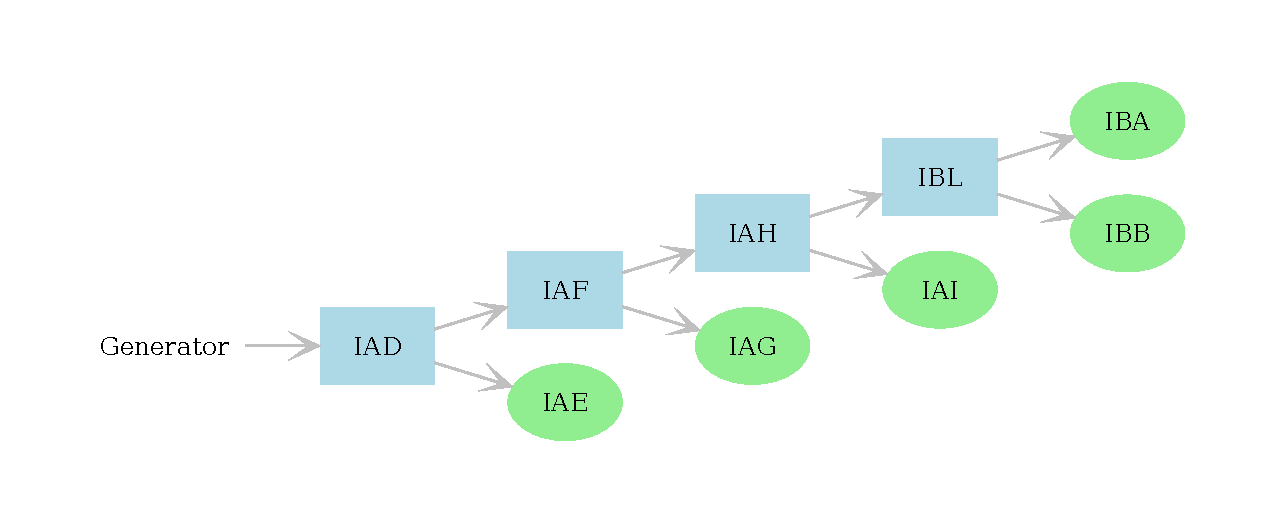
\includegraphics[scale=.7]{subtree.pdf}
%   \caption{The simulated subtree.  Airways are represented in light blue and acini in light green.}
%   \label{fig:subtree_development}
% \end{figure}

\vspace{2.25em}

\begin{figure}[H]\centering
  \begin{tikzpicture}[node distance=2.3cm]
    \node (GEN) [rectangle, rounded corners, minimum width=1.5cm, minimum height=.75cm, draw=black, fill=green!25] {Generator};
    \node (IAD) [airway, right of=GEN, xshift=.25cm]              {\textsc{IAD}};
    \node (IAF) [airway, right of=IAD]                             {\textsc{IAF}};
    \node (IAH) [airway, right of=IAF]                             {\textsc{IAH}};
    \node (IBL) [airway, right of=IAH]                             {\textsc{IBL}};
    \node (IAE) [acinus, above of=IAD, xshift=.75cm]               {\textsc{IAE}};
    \node (IAG) [acinus, below of=IAF, xshift=.75cm]               {\textsc{IAG}};
    \node (IAI) [acinus, above of=IAH, xshift=.75cm]               {\textsc{IAI}};
    \node (IBA) [acinus, above of=IBL, xshift=.75cm]               {\textsc{IBA}};
    \node (IBB) [acinus, below of=IBL, xshift=.75cm]               {\textsc{IBB}};

    \draw [arrow1] (GEN) -- (IAD);
    \draw [arrow1] (IAD) -- (IAF);
    \draw [arrow1] (IAF) -- (IAH);
    \draw [arrow1] (IAH) -- (IBL);
    \draw [arrow1] (IAD) -- (IAE);
    \draw [arrow1] (IAF) -- (IAG);
    \draw [arrow1] (IAH) -- (IAI);
    \draw [arrow1] (IBL) -- (IBA);
    \draw [arrow1] (IBL) -- (IBB);
  \end{tikzpicture}
  \caption{The simulated subtree. Airways are represented in red,
    acini in blue.}
  \label{fig:subtree_development}
\end{figure}

%%% Local Variables:
%%% mode: LaTeX
%%% TeX-master: "../Thesis"
%%% End:



% In this project, Chaste has been relied upon to generate an anatomical
% surrogate for lungs in premature newborns.

%%% Local Variables:
%%% mode: LaTeX
%%% TeX-master: "../Thesis"
%%% End:

% 6. Results
%   6.1. Anatomical
%   6.2. Mechanical Simulation
\section{Results}
\label{sec:results}

% - Disegno surrogato anatomico dell'albero respiratorio.  (output da
%   ParaView).
% - Grafici: un gradino "sopra" (10) le soglie e uno "sotto" (8) (xlims
%   = (.995, 1.09)).

% Grafici dipendenti dal numero di generazioni (?)

\subsection{Anatomical}
\label{subsec:anatomical_results}

% AGGIUNTA MODIFICA, COMPLETARE
% {\color{red} Completare XX facendo simulazioni}

A CT of a 40-week infant was collected. We segmented and extracted the
centreline of 19 major airways, down to 5$^{\text{th}}$ generation.
We also obtained four lobes.

% Mostra immagine delle vie aeree segmentate (skeletonizzazione della
% centreline) e dei quattro lobi su tre piani (xy, xz, yz).

\begin{figure}[H]\centering
  \subfloat[][x-y plane]{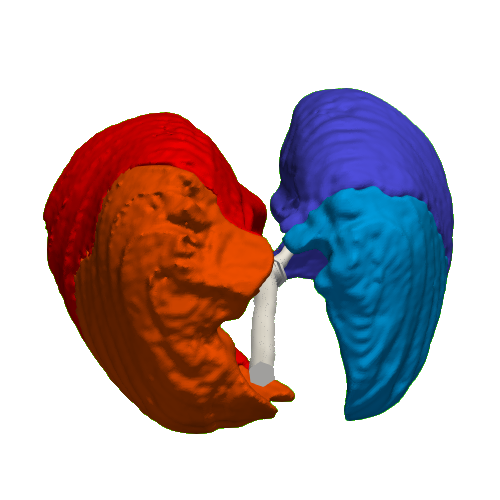
\includegraphics[width=.45\textwidth]{major_airways_xy.png}}%
  \hspace{1cm}
  \subfloat[][y-z plane]{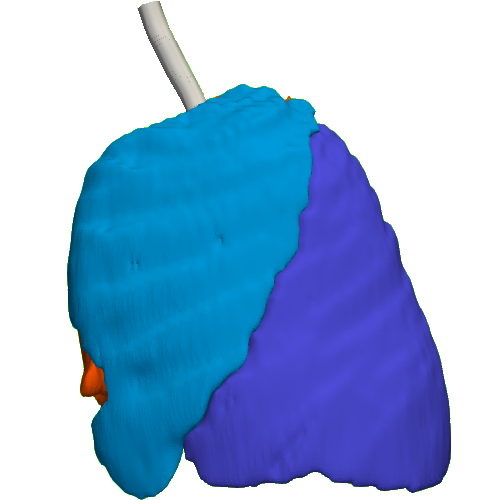
\includegraphics[width=.45\textwidth]{major_airways_yz.png}}\\\vspace{1cm}
  \subfloat[][x-z plane]{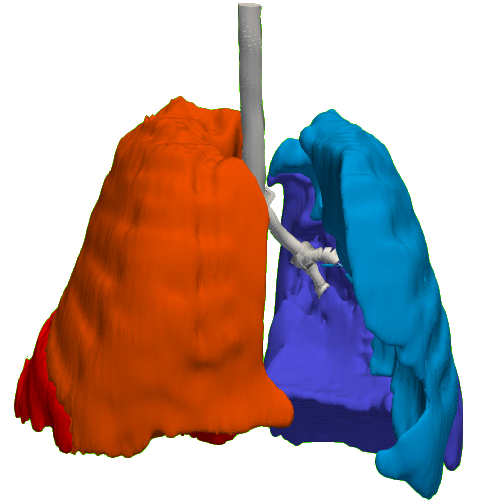
\includegraphics[width=.45\textwidth]{major_airways_xz.png}}

  \caption{Major Airways and Lobes segmentations.  Cyan: Upper Left
    Lung; Blue: Lower Left Lung; Orange: Upper Right Lung; Red: Lower
    Right Lung.}
  \label{fig:anatomical_results}
\end{figure}

Using the developed program, based on the Lung Chaste library, we
reconstructed the missing generations starting from 15000 seed points
per lung.  The obtained airway tree can be displayed by ParaView.
% Mostra immagine dell'albero completo.

\begin{figure}[H]\centering
  \subfloat[][x-y plane]{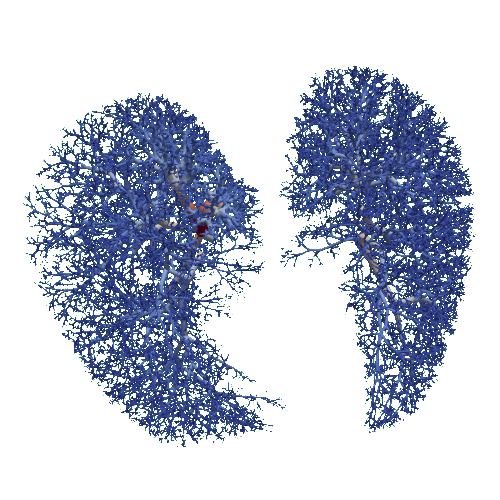
\includegraphics[width=.45\textwidth]{complete_airways_xy.png}}%
  \hspace{1cm}
  \subfloat[][y-z plane]{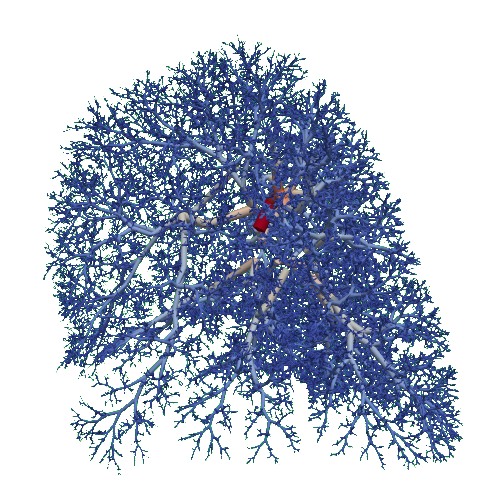
\includegraphics[width=.45\textwidth]{complete_airways_yz.png}}\\\vspace{1cm}
  \subfloat[][x-z plane]{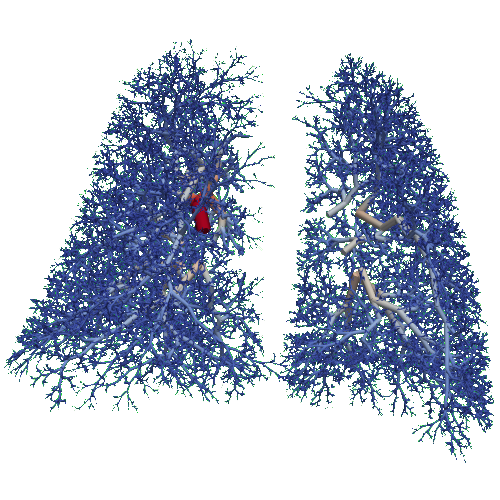
\includegraphics[width=.45\textwidth]{complete_airways_xz.png}}

  \caption{Complete Airways generated by Chaste User Project (major
    airways are here excluded).  They are color-coded with respect to
    their radii.}
  \label{fig:complete_anatomical_results}
\end{figure}

The lobes are fully covered by the statistically generated airways and
this allows us to move a step forward in newborn lung simulation.

\subsection{Mechanical Simulation}
\label{subsec:mechanical_results_subsec}

% Descrizione dei test.  La descrizione della rete in termini di
% parametri va fatta qui?

% Introduzione da aggiungere: lo scopo di queste simulazioni. Queste non
% sono le simulazioni per capire come va il bambino ma per verificare la
% coerenza dei comportamenti dei vari componenti.  Facendo riferimento
% alla figura della sottorete che ho considerato.  Nella sottorete
% abbiamo applicato due livelli diversi di pressione: una sopra la
% pressione capillare, così da aprire tutti i diodi dei vari moduli e
% una sotto la pressione capillare di qualche diodo per vedere le
% differenze.

These simulations are to verify the various components and modules
coherence.  Two tests have been designed as follows.  A step voltage
generator is applied to the electrical equivalent of the newborn lung.
The step amplitude is 10V for the first test and 8V for the second.
In both tests, the step voltage is applied at $t=1$s from the start of
the simulation.

The reason why these values for voltage have been chosen is related
both to the airway subtree described in \Cref{fig:subtree_development}
and to the diode threshold values ``vin\_th'' for airways and acini in
\Cref{tab:airways_test1,tab:acini_test1,tab:airways_test2,tab:acini_test2}.

% Faccio una descrizione di queste curve: si aprono le vie aeree dalla
% più vicina a quella più lontana e gli acini seguono un determinato
% ordine di apertura.

% Quando cambio soglia abbiamo notato che alcuni acini non si aprono
% in quanto la pressione capillare è troppo elevata.  Il fatto di aver
% abbassato la pressione ha rallentato l'apertura di tutti quanti perché
% ci mettono un po' a raggiungere la pressione capillare.  Cambia la
% sequenza di apertura degli acini.  Posso usare nella descrizione dei
% grafici anche i nomi IAE, IAI ecc (facendo però riferimento al
% capitolo in cui introduco il problema).

% AGGIUNTA MODIFICA, COMPLETARE
% To verify the behavior of the mechanical components
% implemented in Julia, we tested the system described by applying

The first test employs a step amplitude for the voltage generator which
overcomes every module diode threshold.  It is possible to check out in
\Cref{fig:mechanical_results_10_1,fig:mechanical_results_8_1} modules
opening times and activation orders.  Airways open from the most
proximal to the most distal one.  It is more interesting to analyze
the activation order of the acini.  They open following a proximal
to distal order but high diode thresholds introduce delays.

% Inserisco gli output di Julia, in particolare correnti e tensioni
% sotto e sopra threshold. (ampiezza scalino di 8 e 10V).
\vspace{2.25em}

\begin{figure}[H]\centering
  \subfloat[][Airways voltages]{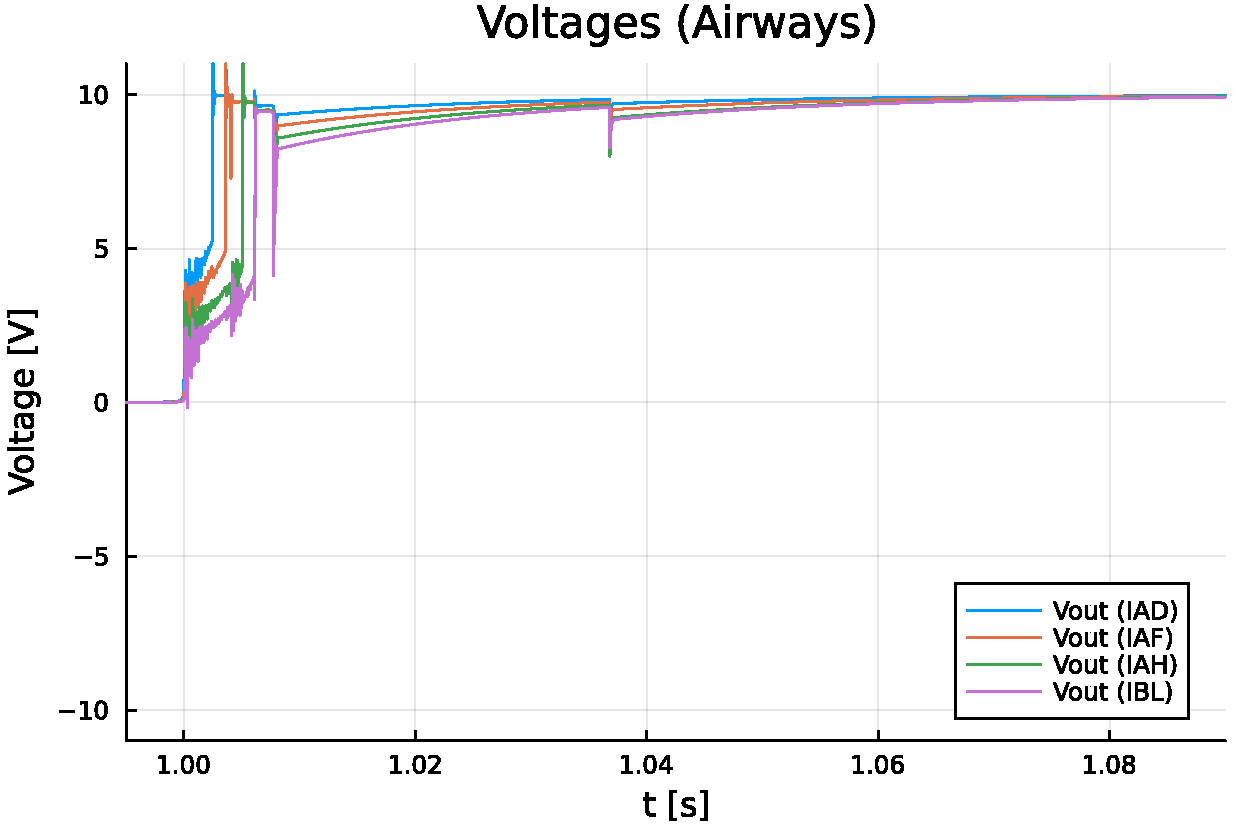
\includegraphics[width=.45\textwidth]{airways_voltages_10.pdf}}%
  \hspace{1cm}
  \subfloat[][Airways currents]{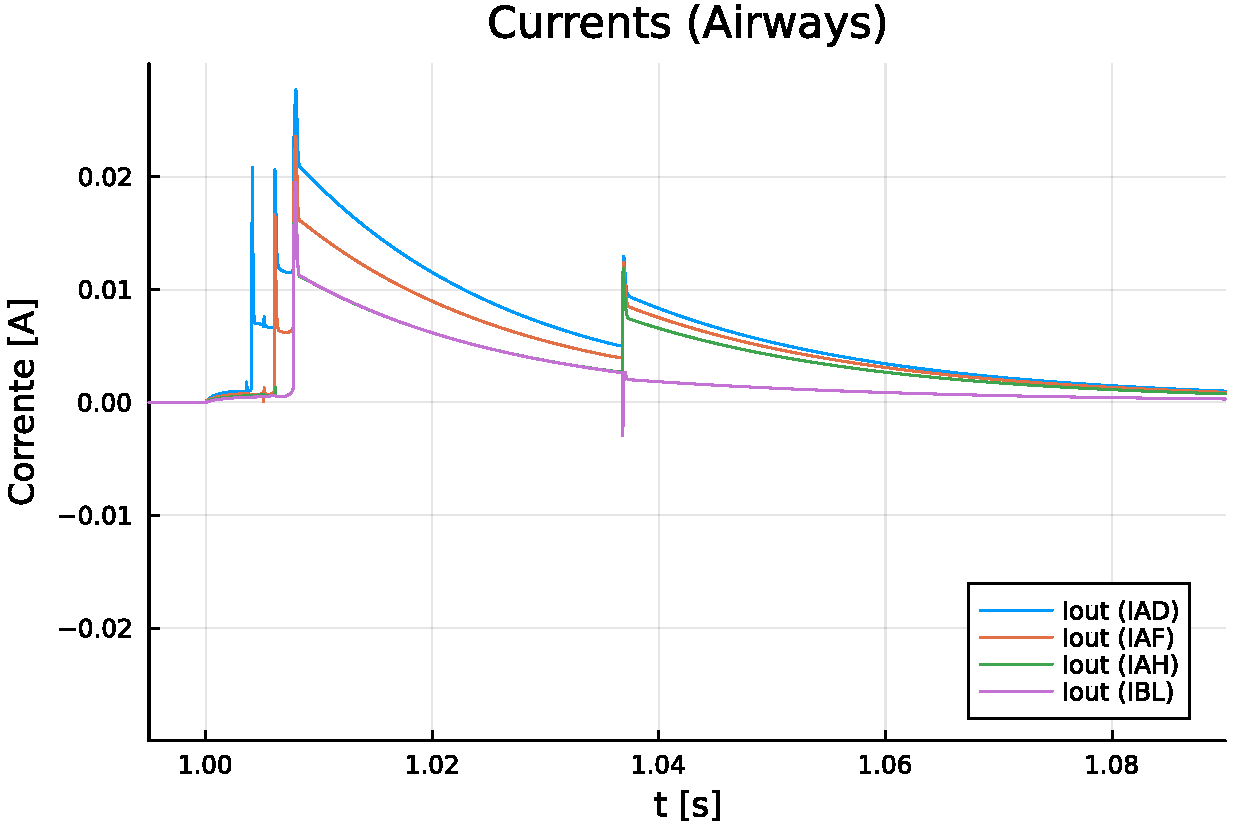
\includegraphics[width=.45\textwidth]{airways_currents_10.pdf}}\\
  \subfloat[][Acini voltages]{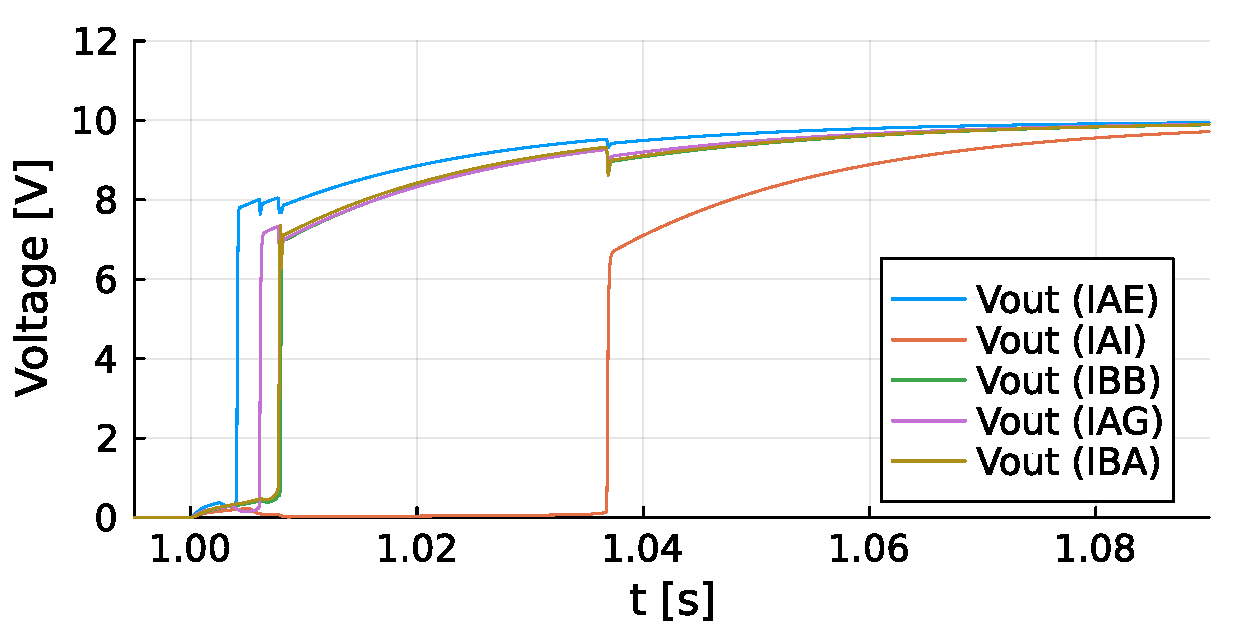
\includegraphics[width=.45\textwidth]{acini_voltages_10.pdf}}%
  \hspace{1cm}
  \subfloat[][Acini currents]{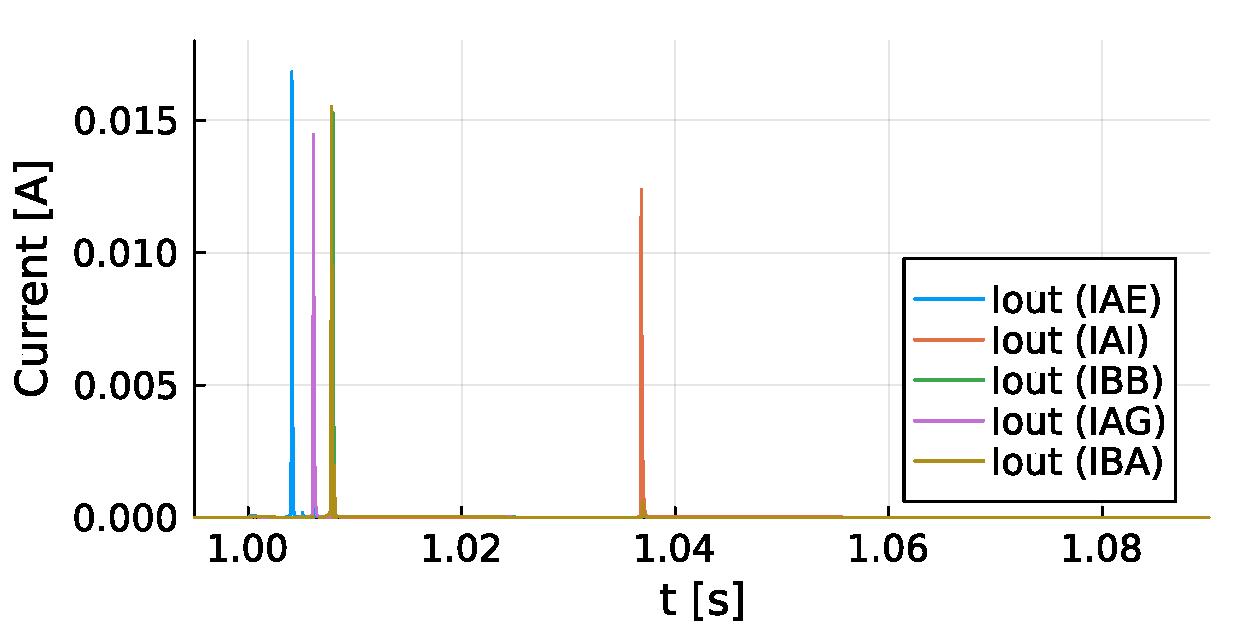
\includegraphics[width=.45\textwidth]{acini_currents_10.pdf}}
  \caption{(Electrically equivalent) mechanical simulation for acini
    and airways.  The step amplitude is 10V.}
  \label{fig:mechanical_results_10_2}
\end{figure}

% Test 1
%% Airways
\begin{table}[H]
  \centering
  \begin{minipage}[h]{.25\textwidth}\centering
    \begin{figure}[H]\centering
  \begin{tikzpicture}[node distance=1.5cm]
    \node (GEN) [rectangle, rounded corners, minimum width=1.5cm, minimum height=.75cm, draw=black, fill=green!25] {Step (10V)};
    \node (IAD) [airway_vertical, below of=GEN]                                                                    {1$^\circ$};
    \node (IAF) [airway_vertical, below of=IAD]                                                                    {2$^\circ$};
    \node (IAH) [airway_vertical, below of=IAF]                                                                    {4$^\circ$};
    \node (IBL) [airway_vertical, below of=IAH]                                                                    {5$^\circ$};
    \node (IAE) [acinus_vertical, left of=IAD, xshift=-.25cm, yshift=-1.5cm]                                       {3$^\circ$};
    \node (IAG) [acinus_vertical, right of=IAF, xshift=.25cm, yshift=-1.5cm]                                       {6$^\circ$};
    \node (IAI) [acinus_vertical, left of=IAH, xshift=-.25cm, yshift=-1.5cm]                                       {9$^\circ$};
    \node (IBA) [acinus_vertical, right of=IBL, xshift=.25cm, yshift=-1.5cm]                                       {7$^\circ$};
    \node (IBB) [acinus_vertical, left of=IBL, xshift=-.25cm, yshift=-1.5cm]                                       {8$^\circ$};

    \draw [arrow1] (GEN) -- (IAD);
    \draw [arrow1] (IAD) -- (IAF);
    \draw [arrow1] (IAF) -- (IAH);
    \draw [arrow1] (IAH) -- (IBL);
    \draw [arrow1] (IAD) -- (IAE);
    \draw [arrow1] (IAF) -- (IAG);
    \draw [arrow1] (IAH) -- (IAI);
    \draw [arrow1] (IBL) -- (IBA);
    \draw [arrow1] (IBL) -- (IBB);
  \end{tikzpicture}
  % \caption{The simulated subtree. Airways are represented in red,
    % acini in yellow.}
  \label{fig:subtree_development_10}
\end{figure}

%%% Local Variables:
%%% mode: LaTeX
%%% TeX-master: "../Thesis"
%%% End:

  \end{minipage}\hspace{1.5cm}
  \begin{minipage}[h]{.6\textwidth}
    {\renewcommand{\arraystretch}{1.2}
      \begin{tabularx}{\textwidth}{|P{6em}|C|C|C|C|}
        \hline
        \rowcolor{red!40}
        \textsc{Airways}
        & IAD
        & IAF
        & IAH
        & IBL\\
        \hline
        \rowcolor{yellow!40}$V_{\text{in,th}}$ [V]
        & 4.67
        & 4.99
        & 5.29
        & 5.59\\
        \hline
        \rowcolor{yellow!40}$T_{\text{open}}$ [s]
        & 1.00246
        & 1.00356
        & 1.00501
        & 1.00611\\
        \hline
        \rowcolor{orange!40}Activ. order
        & 1$^{\circ}$
        & 2$^{\circ}$
        & 4$^{\circ}$
        & 5$^{\circ}$\\
        \hline
      \end{tabularx}
    }
    \caption{Airways opening times and orders when test \#1 is
      performed.}
    \label{tab:airways_test1}
    \vspace{.9cm}
    
    {\renewcommand{\arraystretch}{1.2}
      \begin{tabularx}{\textwidth}{|P{6em}|C|C|C|C|C|}
        \hline
        \rowcolor{blue!25}
        \textsc{Acini}
        & IAE
        & IAG
        & IAI
        & IBA
        & IBB\\
        \hline
        \rowcolor{yellow!40}$V_{\text{in,th}}$ [V]
        & 7.96
        & 8.69
        & 9.25
        & 6.79
        & 7.01\\
        \hline
        \rowcolor{yellow!40}$T_{\text{open}}$ [s]
        & 1.0041
        & 1.0062
        & 1.0369
        & 1.0078
        & 1.0080\\
        \hline
        \rowcolor{orange!40}Activ. order
        & 3$^{\circ}$
        & 6$^{\circ}$
        & 9$^{\circ}$
        & 7$^{\circ}$
        & 8$^{\circ}$\\
        \hline
      \end{tabularx}
    }
    \caption{Acini opening times and orders when test \#1 is
      performed.}
    \label{tab:acini_test1}
  \end{minipage}
  \captionof{figure}{Results summary for test \#1.  On the left, the
    subtree morphology containing the opening order of each module.
    On the right, \Cref{tab:airways_test1,tab:acini_test1} display
    diode thresholds and opening times.}
  \label{fig:mechanical_results_10_1}
\end{table}

% %% Acini
% \begin{table}[H]\centering
%   {\renewcommand{\arraystretch}{1.2}
%     \begin{tabularx}{\textwidth}{|P{6em}|C|C|C|C|C|}
%       \hline
%       \rowcolor{bluePoli!40}
%       \textsc{Acini}
%       & IAE
%       & IAG
%       & IAI
%       & IBA
%       & IBB\\
%       \hline
%       \rowcolor{yellow!40}$V_{\text{in,th}}$ [V]
%       & 7.96
%       & 8.69
%       & 9.25
%       & 6.79
%       & 7.01\\
%       \hline
%       \rowcolor{yellow!40}$T_{\text{open}}$ [s]
%       & 1.00411
%       & 1.00616
%       & 1.03686
%       & 1.00781
%       & 1.00796\\
%       \hline
%       \rowcolor{orange!40}Activ. order
%       & 3$^{\circ}$
%       & 6$^{\circ}$
%       & 9$^{\circ}$
%       & 7$^{\circ}$
%       & 8$^{\circ}$\\
%       \hline
%     \end{tabularx}
%   }
%   \caption{Acini opening times values and total activation order
%     when test \#1 is performed.}
%   \label{tab:acini_test1}
% \end{table}

\clearpage
The second test provides a voltage capable of opening some modules
constituting the subtree.  Opening times and activation orders are
summarized into \Cref{tab:airways_test2,tab:acini_test2}.  Relative
airway activation order is increasing from proximal to distal.  Only
distal acini are activated due to their lower diode thresholds, the
rest remain closed.
\vspace{1.05em}

\begin{figure}[H]\centering
  \subfloat[][Airways voltages]{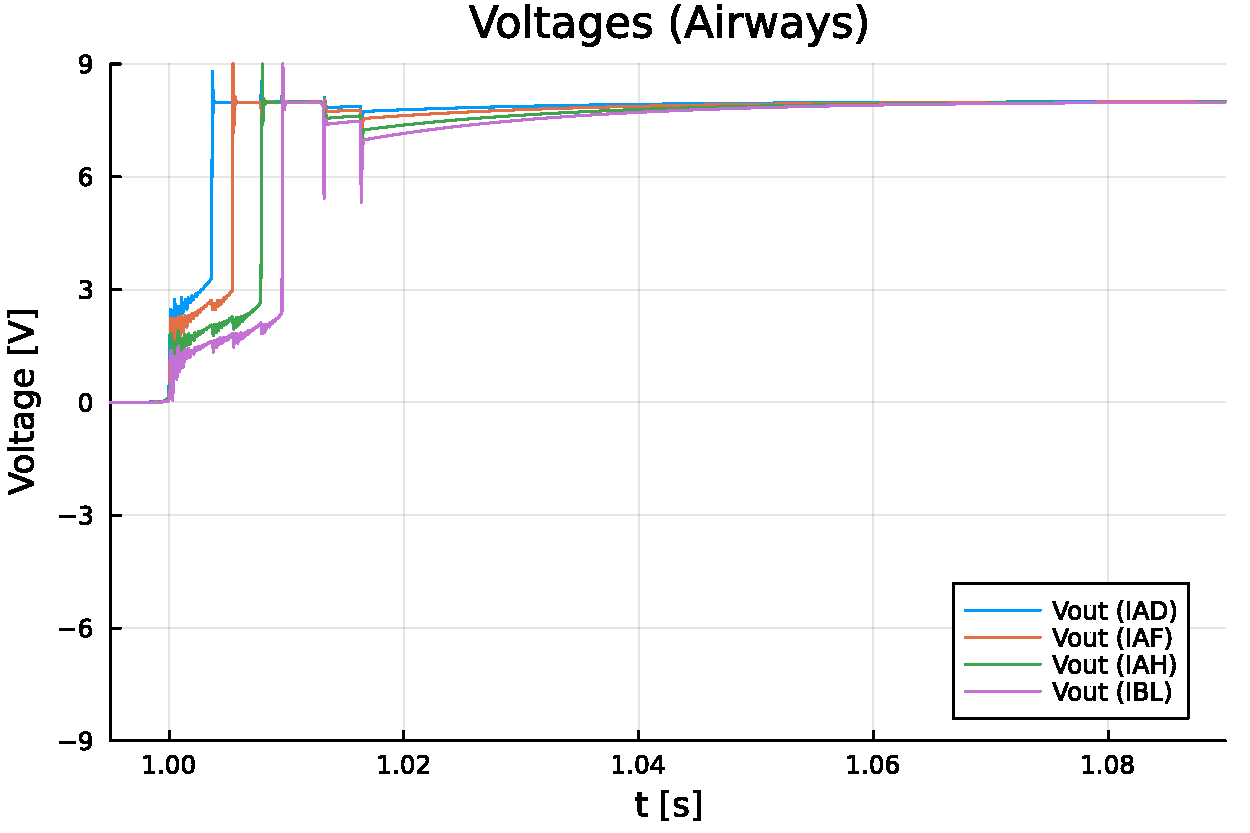
\includegraphics[width=.45\textwidth]{airways_voltages_8.pdf}}%
  \hspace{1cm}
  \subfloat[][Airways currents]{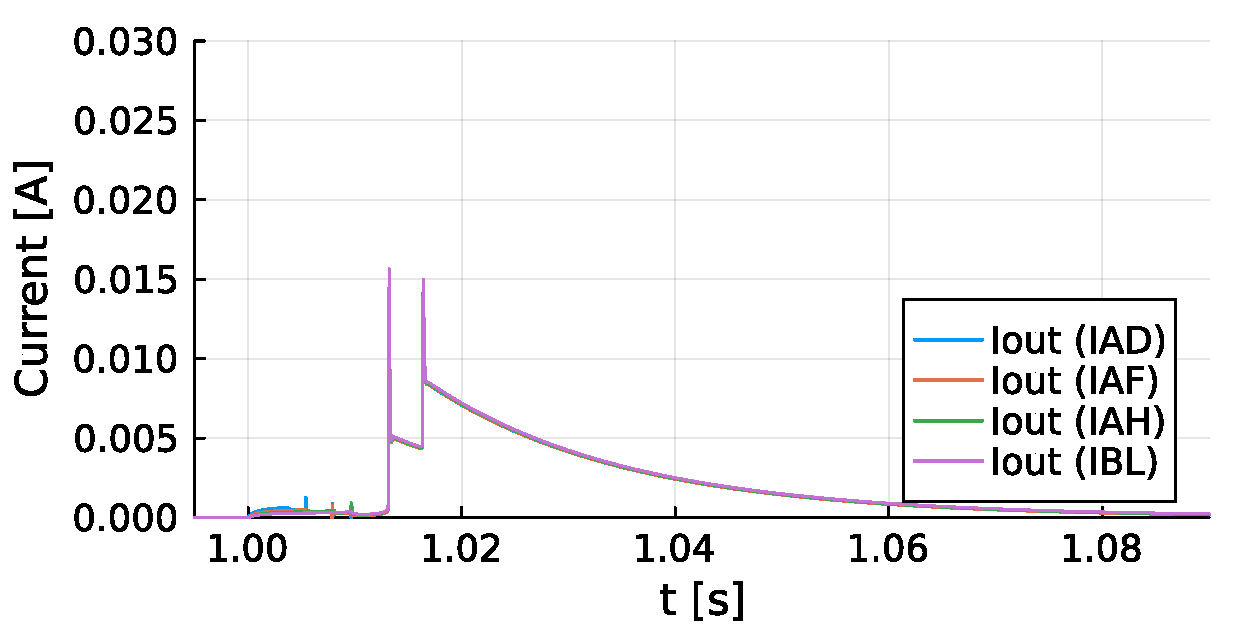
\includegraphics[width=.45\textwidth]{airways_currents_8.pdf}}\\
  \subfloat[][Acini voltages]{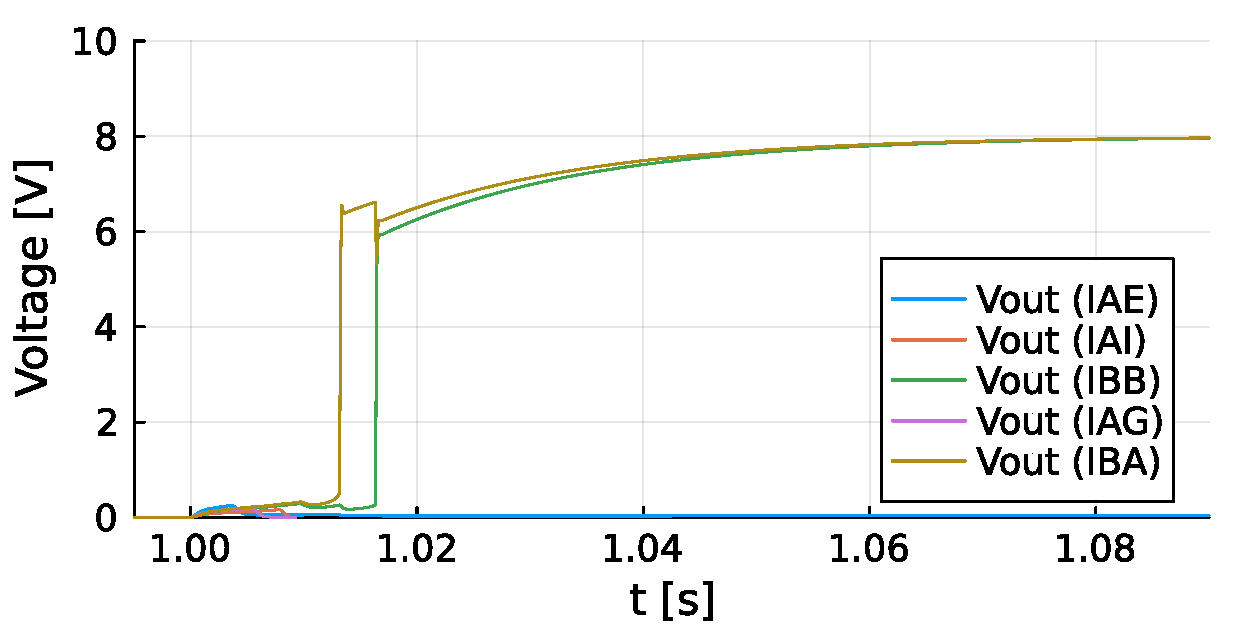
\includegraphics[width=.45\textwidth]{acini_voltages_8.pdf}}%
  \hspace{1cm}
  \subfloat[][Acini currents]{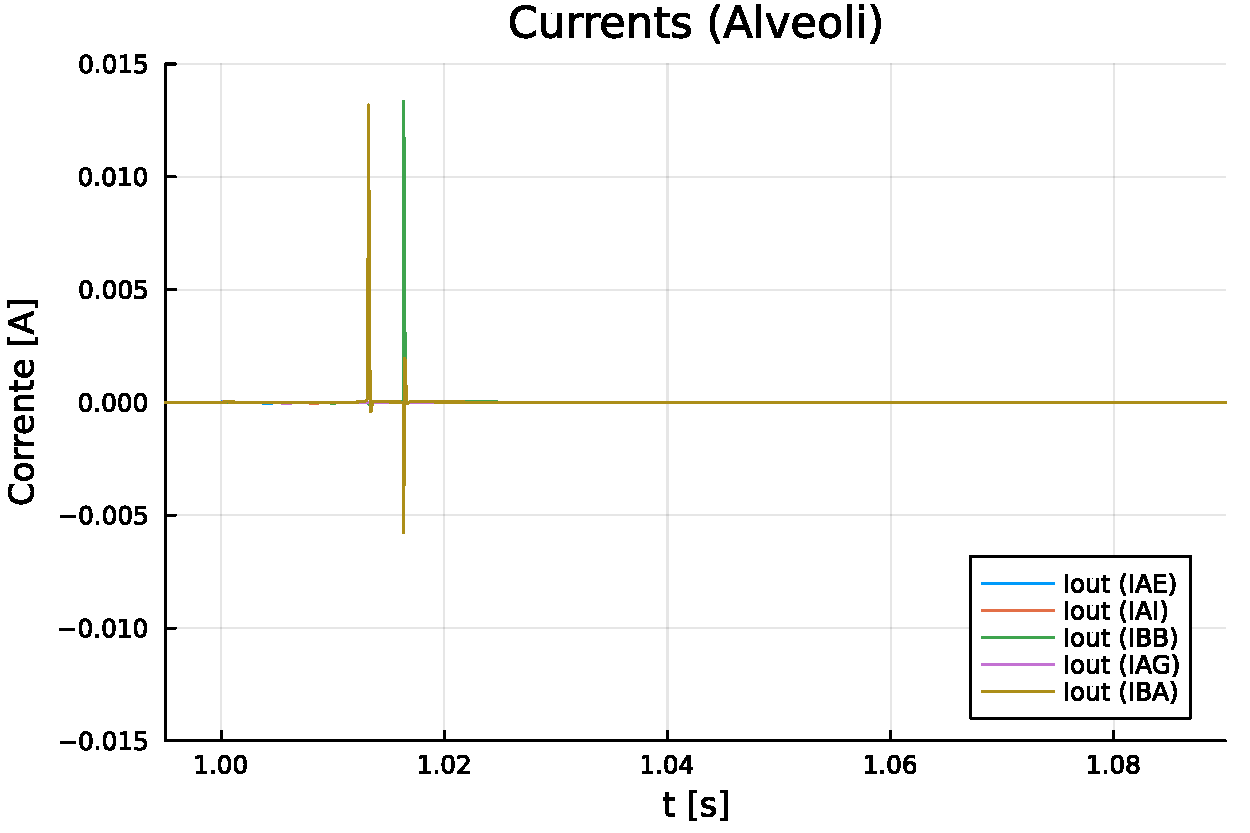
\includegraphics[width=.45\textwidth]{acini_currents_8.pdf}}
  \caption{(Electrically equivalent) mechanical simulation for acini
    and airways.  The step amplitude is 8V.}
  \label{fig:mechanical_results_8_2}
\end{figure}

% Test 2
%% Airways
\begin{table}[H]\centering
  \begin{minipage}{.25\textwidth}\centering
    \begin{figure}[H]\centering
  \begin{tikzpicture}[node distance=1.5cm]
    \node (GEN) [rectangle, rounded corners, minimum width=1.5cm, minimum height=.75cm, draw=black, fill=green!25] {Step (8V)};
    \node (IAD) [airway_vertical, below of=GEN]                                                                    {1$^\circ$};
    \node (IAF) [airway_vertical, below of=IAD]                                                                    {2$^\circ$};
    \node (IAH) [airway_vertical, below of=IAF]                                                                    {3$^\circ$};
    \node (IBL) [airway_vertical, below of=IAH]                                                                    {4$^\circ$};
    \node (IAE) [acinus_vertical, left of=IAD, xshift=-.25cm, yshift=-1.5cm]                                       {---};
    \node (IAG) [acinus_vertical, right of=IAF, xshift=.25cm, yshift=-1.5cm]                                       {---};
    \node (IAI) [acinus_vertical, left of=IAH, xshift=-.25cm, yshift=-1.5cm]                                       {---};
    \node (IBA) [acinus_vertical, right of=IBL, xshift=.25cm, yshift=-1.5cm]                                       {5$^\circ$};
    \node (IBB) [acinus_vertical, left of=IBL, xshift=-.25cm, yshift=-1.5cm]                                       {6$^\circ$};

    \draw [arrow1] (GEN) -- (IAD);
    \draw [arrow1] (IAD) -- (IAF);
    \draw [arrow1] (IAF) -- (IAH);
    \draw [arrow1] (IAH) -- (IBL);
    \draw [arrow1] (IAD) -- (IAE);
    \draw [arrow1] (IAF) -- (IAG);
    \draw [arrow1] (IAH) -- (IAI);
    \draw [arrow1] (IBL) -- (IBA);
    \draw [arrow1] (IBL) -- (IBB);
  \end{tikzpicture}
  % \caption{The simulated subtree. Airways are represented in red,
    % acini in yellow.}
  \label{fig:subtree_8_development}
\end{figure}

%%% Local Variables:
%%% mode: LaTeX
%%% TeX-master: "../Thesis"
%%% End:

  \end{minipage}\hspace{1.5cm}
    \begin{minipage}{.6\textwidth}\centering
    {\renewcommand{\arraystretch}{1.2}
      \begin{tabularx}{\textwidth}{|P{6em}|C|C|C|C|}
        \hline
        \rowcolor{red!40}
        \textsc{Airways}
        & IAD
        & IAF
        & IAH
        & IBL\\
        \hline
        \rowcolor{yellow!40}$V_{\text{in,th}}$ [V]
        & 4.67
        & 4.99
        & 5.29
        & 5.59\\
        \hline
        \rowcolor{yellow!40}$T_{\text{open}}$ [s]
        & 1.00361
        & 1.00536
        & 1.00781
        & 1.00961\\
        \hline
        \rowcolor{orange!40}Activ. order
        & 1$^{\circ}$
        & 2$^{\circ}$
        & 3$^{\circ}$
        & 4$^{\circ}$\\
        \hline
      \end{tabularx}
    }
    \caption{Airways opening times and orders when test \#2 is
      performed.}
    \label{tab:airways_test2}
    \vspace{.9cm}
    {\renewcommand{\arraystretch}{1.2}
      \begin{tabularx}{\textwidth}{|P{6em}|C|C|C|C|C|}
        \hline
        \rowcolor{blue!25}
        \textsc{Acini}
        & IAE
        & IAG
        & IAI
        & IBA
        & IBB\\
        \hline
        \rowcolor{yellow!40}$V_{\text{in,th}}$ [V]
        & 7.96
        & 8.69
        & 9.25
        & 6.79
        & 7.01\\
        \hline
        \rowcolor{yellow!40}$T_{\text{open}}$ [s]
        & $+\infty$
        & $+\infty$
        & $+\infty$
        & 1.01316
        & 1.01636\\
        \hline
        \rowcolor{orange!40}Activ. order
        & ---
        & ---
        & ---
        & 5$^{\circ}$
        & 6$^{\circ}$\\
        \hline
      \end{tabularx}
      \caption{Acini opening times values and total activation order
        when test \#2 is performed.}
      \label{tab:acini_test2}
    }
  \end{minipage}
  \captionof{figure}{Results summary for test \#2.  On the left, the
    subtree morphology containing the opening order of each module.
    On the right, \Cref{tab:airways_test2,tab:acini_test2} display
    diode thresholds and opening times. Long dashes: no opening has
    occurred.}
  \label{fig:mechanical_results_8_1}
\end{table}

% %% Acini
% \begin{table}[H]\centering
% \end{table}

%%% Local Variables:
%%% mode: LaTeX
%%% TeX-master: "../Thesis"
%%% End:

% 7. Discussion and Conclusion
\section{Discussion and Conclusion}

As future development it is possible to edit properly airway
generation parameters in order to better approximate the target
morphometric characteristics, so to be able to produce a
patient-specific anatomical model.  This allows for gathering more
accurate mechanical parameters for the simulation phase.

%%% Local Variables:
%%% mode: LaTeX
%%% TeX-master: "../Thesis"
%%% End:


%-----------------------------------------------------------------------------
% BIBLIOGRAPHY
%-----------------------------------------------------------------------------
\printbibliography

%-----------------------------------------------------------------------------
% APPENDICES
%-----------------------------------------------------------------------------
% \appendix
% \section{Appendix A}
If you need to include an appendix to support the research in your
thesis, you can place it at the end of the manuscript.  An appendix
contains supplementary material (figures, tables, data, codes,
mathematical proofs, surveys, \dots) which supplement the main results
contained in the previous sections.


% \section{Appendix B}
It may be necessary to include another appendix to better organize the
presentation of supplementary material.



% \begin{figure}[H]\centering
  \begin{circuitikz}[]
    % Circuit
    %% Main branch

    %%% Input Node
    \draw (1.5,0)
    node[ocirc] (circuit_IN) {}
    to[short, i=$i_{\text{in}}$, -*] ++(1.5,0) coordinate(D_SW_IN)
    ;
    
    %%% Diode // Switch branch
    \draw (D_SW_IN)
    to[short] ++(0,.5)
    to[diode, v^<=$V_{\text{in,th}}$, color=bluePoli] ++(2,0) coordinate(D_SW_OUT)
    to[short, -*] (D_SW_IN-|D_SW_OUT)
    ;
    \draw (D_SW_IN)
    to[short] ++(0,-.5)
    to[switch, color=bluePoli, a_=$\left(V_{\text{in}}\geq V_{\text{in,th}}\right) \lor \left(V_{\text{in}} \text{ = } 0\right)$] ++(2,0)
    to[short] (D_SW_IN-|D_SW_OUT)
    ;

    %% Main branch
    \draw (D_SW_IN-|D_SW_OUT)
    to[short] ++(.5,0)
    to[variable resistor, color=bluePoli, l=$R_{\text{tube}} / 2$] ++(2,0)
    to[variable inductor, color=bluePoli, l=$I_{\text{tube}} / 2$] ++(2,0) coordinate (C_g_IN)
    to[short] ++(1.5,0) coordinate (SW_IN)
    to[variable resistor, color=bluePoli, l=$R_{\text{tube}} / 2$] ++(2,0)
    to[variable inductor, color=bluePoli, l=$I_{\text{tube}} / 2$] ++(2,0)
    to[short, i=$i_{\text{out}}$] ++(1,0)
    node[ocirc] (circuit_OUT) {}
    ;

    %%% C_g branch
    \draw (C_g_IN)
    to[C=$C_{\text{g}}$, *-] ++(0,-3.5)
    node[ground]{} ++(0,0)
    ;

    %%% Sw branch
    \draw (SW_IN)
    to[L=$I_{\text{sw}}$, *-] ++(0,-1.5)
    to[R=$R_{\text{sw}}$] ++(0,-1)
    to[C=$C_{\text{sw}}$] ++(0,-1)
    node[ground]{} ++(0,0)
    ;
    
    %% Open circuit (input)
    \draw (circuit_IN)
    to[open, -o, v<=$V_{\text{in}}$] ++(0, -3.5)
    node[ground] {}
    ;
    %% Open circuit (output)
    \draw (circuit_OUT)
    to[open, -o, v^<=$V_{\text{out}}$] ++(0, -3.5)
    node[ground] {}
    ;

    % Nodes
    %% IN
    \draw  (circuit_IN.west)
    node[draw, anchor=east, color=white, fill=bluePoli!50] (node_IN) {IN}
    ;
    % \draw (node_IN.east) node[ocirc, right]{}
    % ;
    %% OUT
    \draw  (circuit_OUT.east)
    node[draw, anchor=west, color=white, fill=bluePoli!50] (node_OUT) {OUT}
    ;
  \end{circuitikz}
  \caption{Airway equivalent circuit.  In blue: all current integral-dependent components.}
  \label{fig:airway}

\end{figure}

%%% Local Variables:
%%% mode: LaTeX
%%% TeX-master: "../Thesis"
%%% End:

% \begin{figure}[H]\centering
  \begin{circuitikz}[scale=.9]
    % Circuit
    %% Main branch

    %%% Input Node
    \draw (1.5,0)
    node[ocirc] (circuit_IN) {}
    to[short, i=$i_{\text{in}}$, -*] ++(1.5,0) coordinate(D_SW_IN)
    ;
    
    %%% Diode // Switch branch
    \draw (D_SW_IN)
    to[short] ++(0,.5)
    to[diode, v^<=$V_{\text{in,th}}$, color=bluePoli] ++(2,0) coordinate(D_SW_OUT)
    to[short, -*] (D_SW_IN-|D_SW_OUT)
    ;
    \draw (D_SW_IN)
    to[short] ++(0,-.5)
    to[switch, color=bluePoli, a_=$\left(V_{\text{in}}\geq V_{\text{in,th}}\right) \lor \left(V_{\text{in}} \text{ = } 0\right)$] ++(2,0)
    to[short] (D_SW_IN-|D_SW_OUT)
    ;

    %% Main branch
    \draw (D_SW_IN-|D_SW_OUT)
    % to[short] ++(.5,0)
    to[variable resistor, color=bluePoli, l=$R_{\text{tube}}$] ++(2.25,0)
    to[variable inductor, color=bluePoli, l=$I_{\text{tube}}$] ++(2.25,0) coordinate (circuit_OUT)
    % to[short] ++(.5,0)
    to[L=$I_{\text{t}}$] ++(2.25,0)
    to[R=$R_{\text{t}}$] ++(1.5,0)
    to[C=$C_{\text{t}}$] ++(1.5,0) coordinate (S_IN)
    % node[ocirc] (circuit_OUT) {}
    ;

    \draw (S_IN)
    to[short] ++(0,-.5)
    to[R, l_=$R_{\text{s}}$] ++(2,0)
    to[short] ++(0,.5)
    ;
    \draw (S_IN)
    to[short, *-] ++(0,.5)
    to[C=$C_{\text{s}}$] ++(2,0)
    to[short] ++(0,-.5)
    to[short, *-] ++(.5,0)
    node[ground]{} ++(0,0)
    ;

    %%% C_g branch
    \draw (circuit_OUT) node[draw, anchor=south, color=white, fill=bluePoli!50] {OUT}
    to[C=$C_{\text{g}}$, i=$i_{\text{out}}$, v<=$V_{\text{out}}$, *-] ++(0,-3.5)
    node[ground]{} ++(0,0)
    ;

    %% Open circuit (input)
    \draw (circuit_IN)
    to[open, -o, v<=$V_{\text{in}}$] ++(0, -3.5)
    node[ground] {}
    ;
    % %% Open circuit (output)
    % \draw (circuit_OUT)
    % {[red!60] to[open, -o, v^<=$V_{\text{out}}$] ++(0, -3.5)}
    % node[ground] {}
    % ;

    % Nodes
    %% IN
    \draw  (circuit_IN.west)
    node[draw, anchor=east, color=white, fill=bluePoli!50] (node_IN) {IN}
    ;
    % \draw (node_IN.east) node[ocirc, right]{}
    % ;
    %% OUT

  \end{circuitikz}
  \caption{Alveolus equivalent circuit.  In blue: all current integral-dependent components.}
  \label{fig:alveolus}

\end{figure}


%%%%%%%%%%%%%%%%%%%%%%%%%%%%%%%%%%%%%%%%%%%%%%%%%%%%%%%%%%%%%%
%%     ABSTRACT IN ITALIAN LANGUAGE AND ACKNOWLEDGMENTS     %%
%%%%%%%%%%%%%%%%%%%%%%%%%%%%%%%%%%%%%%%%%%%%%%%%%%%%%%%%%%%%%%
\cleardoublepage

%-----------------------------------------------------------------------------
% SOMMARIO
%-----------------------------------------------------------------------------
\section*{Abstract in lingua italiana}
Durante la gravidanza, le vie aeree del feto sono riempite di un
liquido noto come liquido polmonare fetale, essenziale per lo sviluppo
della larghezza delle vie aeree. Di conseguenza, alla nascita, il
sistema respiratorio deve espellere questo liquido per permettere
l'entrata e l'uscita dell'aria, un processo necessario per la
respirazione (aerazione). Il riassorbimento del liquido inizia qualche
giorno prima del parto attraverso processi chimici che coinvolgono i
canali del sodio e, durante il parto naturale, il liquido viene
espulso dalla bocca e dal naso grazie alla compressione del torace del
neonato. Nei neonati a termine, la probabilità di complicazioni
durante l'aerazione è molto bassa. Tuttavia, lo scenario è molto
diverso per i neonati pretermine, che nascono prima delle 37 settimane
di gestazione rispetto alle tipiche 40 settimane di una gravidanza
normale.  Sebbene le manovre di reclutamento abbiano suscitato un
maggiore interesse nella ventilazione dei pretermine, non esiste
ancora una strategia medica comune. Le procedure sperimentali vengono
testate sugli animali, presentando sfide nel ottenere risultati a
causa dell'invasività delle procedure e dei problemi etici
associati. La modellizzazione in silico del polmone adulto è stata
utile per comprendere la patofisiologia e fare diagnosi. Pertanto, lo
stesso approccio potrebbe aiutare ad analizzare le diverse strategie
di reclutamento e il loro impatto sul polmone durante l'aerazione
iniziale alla nascita. Tuttavia, i modelli in silico dei polmoni
neonatali sono limitati alla descrizione fino alla prima generazione
dell'albero bronchiale e, pertanto, non sono adeguati a simulare i
cambiamenti fisiologici che avvengono alla nascita.  \vspace{15pt}

% Vedi sommario di Mani20.

\begin{tcolorbox}[arc=0pt, boxrule=0pt, colback=bluePoli!60, width=\textwidth, colupper=white]
  \textbf{Parole chiave:} modello morfometrico, processo di aerazione, polmone, neonato, sistema respiratorio
\end{tcolorbox}


%-----------------------------------------------------------------------------
% ACKNOWLEDGEMENTS
%-----------------------------------------------------------------------------
% \section*{Acknowledgements}

Vorrei innanzitutto ringraziare il Professor Raffaele Dellaca' e la
Dott.ssa Chiara Veneroni per l'opportunità di lavorare in laboratorio
e per il loro grande aiuto in questi mesi, dalla fase di progettazione
a quella di scrittura.  Ringrazio gli studenti e i dottorandi di
«TechRes» per tutti i consigli e i bei momenti trascorsi insieme.

Un ringraziamento speciale va alla Dott.ssa Francesca Pennati, al
Dott. Cavigioli, e al Dott. Campari per il loro contributo nella fase
di Image Processing.

Un grazie particolare alla mia famiglia, senza la quale non avrei
avuto il privilegio di frequentare l'Università che desideravo.  In
particolare, dedico un pensiero a mio nonno che oggi non può essere
presente ma che potrà leggere il manoscritto in seguito.  Vi porto
sempre nel cuore.

Ringrazio di cuore Noemi che mi ha incoraggiato nei momenti di
difficoltà.

Ringrazio calorosamente gli amici, di una vita e nuovi.

Un grazie anche a tutti coloro che hanno anche solo minimamente
creduto in me.

Grazie a tutti, non sarebbe stato lo stesso senza ciascuno di voi.

%%% Local Variables:
%%% mode: LaTeX
%%% TeX-master: "../Thesis"
%%% End:


\end{document}

%%% Local Variables:
%%% mode: LaTeX
%%% TeX-master: t
%%% End:
